\documentclass[12pt]{report}

\usepackage{graphics}
\usepackage{tabularx}
\usepackage{blindtext}
\usepackage[a4paper,pdftex,hmargin=0.75in,vmargin={1.1in,0.6in},head=75pt,foot=45pt, left=2.5cm, right=2.5cm, includefoot, footskip=60pt]{geometry}


\makeatletter
\newcommand\frontmatter{%
    \cleardoublepage
  %\@mainmatterfalse
  \pagenumbering{roman}}
\newcommand\mainmatter{%
    \cleardoublepage
 % \@mainmattertrue
  \pagenumbering{arabic}}

\newcommand\backmatter{%
  \if@openright
    \cleardoublepage
  \else
    \clearpage
  \fi
 % \@mainmatterfalse
  }
\makeatother

\makeatletter
\setlength{\@fptop}{0pt}
\makeatother

%\renewcommand*\ShowFrameColor{\color{red}}
%\usepackage[square,numbers, sort&compress]{natbib}
%%%%%%%%%%%%%%%%%%%%%%%%%%%%%%%%%%%%%%%%%%%%%%%%%%%%%%%%
\usepackage{comment}
\usepackage{etoolbox}
\usepackage{supertabular}
\usepackage{graphicx}
\usepackage{color,soul}
\usepackage{booktabs}
\usepackage{makecell}
\renewcommand\theadfont{\bfseries}
%\usepackage{cite}
\usepackage{verbatim}
\usepackage{paralist}
\usepackage{algorithmicx}
\usepackage{algorithm}
\usepackage[noend]{algpseudocode}
\usepackage{hvfloat}
\usepackage{enumitem}
\usepackage{comment}
\usepackage{chngpage}
\usepackage[bottom]{footmisc}
\usepackage{url}
\usepackage{microtype}
\usepackage[utf8]{inputenc}
\usepackage[english]{babel}
\usepackage{csquotes}
\usepackage[table,dvipsnames]{xcolor}
\usepackage{lipsum}
\usepackage{afterpage}
%\usepackage{svg}
\usepackage{xcolor}
\usepackage{tabularx}
\usepackage{wallpaper}
\usepackage{adjustbox}
\usepackage[normalem]{ulem}
\useunder{\uline}{\ul}{}
\usepackage{rotating}
\usepackage[pagestyles]{titlesec}
\usepackage{parskip}
\usepackage{listings}
\lstset{language=C,breaklines=true}
\usepackage{amsmath}
\usepackage{amsfonts}
\usepackage{amssymb}
\usepackage[justification=centering, style=base]{caption}
\usepackage{fontenc}
\usepackage{multicol}
\usepackage{multirow}
\usepackage{mathptmx}
\usepackage{array}
\usepackage{relsize}
\usepackage{subcaption}
\captionsetup[subfigure]{textfont=normalfont,singlelinecheck=off,justification=centerfirst, format=hang}
\usepackage{tcolorbox}
\usepackage{lscape}
\usepackage{lastpage}
\usepackage[natbib=true, style=numeric-comp, maxbibnames=99, sorting=none, url=false, doi=false, isbn=false]{biblatex}
\AtEveryBibitem{
    \clearfield{urlyear}
    \clearfield{urlmonth}
    \clearfield{note}
    \clearfield{eprint}
    \clearfield{url}
    \clearfield{titleaddon}
}
\usepackage{acro}
\setlength{\headsep}{1.5cm}
\usepackage[toc,page]{appendix}
\usepackage[nottoc]{tocbibind} % for show references in toc
\usepackage{pgfgantt}
\frenchspacing
%\usepackage{showframe}% for show page layout
% \usepackage{afterpage}
% \newcommand\myemptypage{
%     \null
%     \thispagestyle{empty}
%     \addtocounter{page}{-1}
%     \newpage
%     }
    
%%%%%%%%%%%%%%%%%
\usepackage[final]{pdfpages}
\patchcmd{\chapter}{\thispagestyle{plain}}{\thispagestyle{fancy}}{}{}
%%%%%%%%%%%%%%%%%%%%%%%%%%%%%%%%%%%%%%%%%%%%%%%%%%%%%%
\usepackage{fancyhdr}
\pagestyle{fancy}
%\fancyhf{}
\lhead{
\includegraphics[height=1.2cm]{fig/UPC.png}}
\rhead{
\includegraphics[height=1.3cm]{fig/Telecos.png}}
\fancyfoot[C]{\thepage{}}
%\fancypagestyle{plain}{%
%\renewcommand{\footrulewidth}{0.4pt}
%\futurelet\TMPfootrule\def\footrule{{\color{upcorange}\TMPfootrule}}
%\futurelet\TMPfootrule\def\footrule{{\color{gray!80}\TMPfootrule}}
\renewcommand{\headrulewidth}{0.4pt}
\renewcommand{\headrule}{\hbox to\headwidth{%
%\color{upcorange}\leaders\hrule height \headrulewidth\hfill}}
\color{gray!80}\leaders\hrule height \headrulewidth\hfill}}
\usepackage[hypertexnames=false]{hyperref}
\hypersetup{
    colorlinks=true,%
    citecolor=black,%
    filecolor=black,%
    linkcolor=black,%
    urlcolor=black
}
\usepackage[capitalise]{cleveref}
% \newcommand{\crefrangeconjunction}{--}
\crefrangelabelformat{equation}%
{(#3#1#4--#5\crefstripprefix{#1}{#2}#6)}
\crefrangelabelformat{subequation}%
{(#3#1#4--#5\crefstripprefix{#1}{#2}#6)}
\crefrangelabelformat{table}%
{(#3#1#4--#5\crefstripprefix{#1}{#2}#6)}
\crefrangelabelformat{figure}%
{(#3#1#4--#5\crefstripprefix{#1}{#2}#6)}
% \crefrangelabelformat{subfigure}%
% {(#3#1#4--#5\crefstripprefix{#1}{#2}#6)}

\bibliography{TexFiles/mylib}
%\addbibresource{TexFiles/mylib.bib}
\renewcommand*{\bibfont}{\small}
\setlength{\bibitemsep}{9pt plus 0.3ex}

\usepackage[acronym,toc,indexonlyfirst]{glossaries}
\makeglossaries




\begin{document}
% \pagenumbering{roman}

\begin{titlepage}
\begin{center}

\includegraphics[scale=1]{fig/ETSETB.png}\vspace{1.2cm}
\mbox{}\\[0pc]

\Large\rmfamily{\textsc{Machine Learning for Sensor Data Processing} \\
\Large\rmfamily{\textsc{in Biomedical Applications}}}\\[36pt]

\large\rmfamily{{\textmd{Master's Thesis}} \\
\large\rmfamily{\textmd{Submitted to the Faculty of the}} \\
\large\rmfamily{\textsl{Escola Tècnica d'Enginyeria de Telecomunicació de Barcelona}}} \\[6pt]

\large\rmfamily{\textbf{Universitat Politècnica de Catalunya}} \\[24pt]

\large\rmfamily{{by}\\
\Large\rmfamily{\textbf{Mani Rezaeirad}}}\\[36pt]

\large\rmfamily{{\textmd{In partial fulfillment}}\\
\large\rmfamily{\textmd{of the requirements for the degree of}}\\
\large\rmfamily{\textmd{Master in Telecommunications Engineering}}}\\[42pt]

      {\large\rmfamily{%
       \begin{tabular}{rlll}
        Supervisors:        & Pierluigi Salvo Rossi & NTNU & IES \\
                            & Veronica Vilaplana Besler  & UPC  & TSC   \\[6pt]
        Co-supervisor:    & Giampiero Salvi  & NTNU  & IES  \\[6pt]
        Advisor:    & Nils Kristian Skjærvold & NTNU  & ISB \\[6pt]
        Co-advisor: & Eline Stenwig & NTNU & ISB \\
        
       \end{tabular}\par
      }\vspace{1.6cm}}


%\vspace{1.1cm}
\normalsize{Barcelona, October 2020}\\
%\noindent\large{Trondheim}\\ 
\end{center}
\end{titlepage}


% \afterpage{\blankpage}
% \newpage
% \thispagestyle{empty} % empty
% \mbox{}
\providecommand\phantomsection

% \addcontentsline{toc}{chapter}{Dedication}
\begin{center}
    {\thispagestyle{empty}
    \itshape
    \vspace*{\fill}
    To my parents, \textbf{Kambiz} and \textbf{Farzaneh}, for their love, support, and encouragement
    \vspace*{\fill}
    }
\end{center}

%\clearpage
%\afterpage{\blankpage}
% \newpage
% \thispagestyle{empty} % empty
% \mbox{}
\providecommand\phantomsection

\pagenumbering{gobble}% Remove page numbers (and reset to 1)

\frontmatter

\tableofcontents
\listoffigures
\listoftables

\newpage
\thispagestyle{empty} % empty
\mbox{}

%\cleardoublepage\phantomsection\addcontentsline{toc}{chapter}{Glossary}
%\chapter*{Glossary}

\newacronym{ML}{ML}{Machine Learning}
\newacronym{ICU}{ICU}{Intensive Care Unit}
\newacronym{ROC}{ROC}{Receiver Operating Characteristic}
\newacronym{AUC}{AUC}{Area Under the ROC Curve}
\newacronym{LDA}{LDA}{Linear Discriminant Analysis}
\newacronym{LR}{LR}{Logistic Regression}
\newacronym{SVM}{SVM}{Support Vector Machine}
\newacronym{NB}{NB}{Na\"ive Bayes}
\newacronym{CART}{CART}{Classification And Regression Tree}
\newacronym{KNN}{KNN}{K-Nearest Neighbors}
\newacronym{NTNU}{NTNU}{Norwegian University of Science and Technology}
\newacronym{UPC}{UPC}{Universitat Politècnica de Catalunya}
\newacronym{eICU}{eICU}{electronic Intensive Care Unit}
\newacronym{XGB}{XGBoost}{eXtreme Gradient Boosting Decision Tree}
\newacronym{HICL}{HICL}{Health Insurance Contract Language}
\newacronym{PRN}{PRN}{pro re nata}
\newacronym{APACHE}{APACHE}{Acute Physiology, Age, and Chronic Health Evaluation}
\newacronym{APS}{APS}{Acute Physiology Score}
\newacronym{SAPS}{SAPS}{Simplified Acute Physiology Score}
\newacronym{SOFA}{SOFA}{Sequential Organ Failure Assessment}
\newacronym{AI}{AI}{Artificial Intelligence}
\newacronym{MIMIC}{MIMIC}{Multiparameter Intelligent Monitoring in Intensive Care}
\newacronym{eICU-CRD}{eICU-CRD}{eICU Collaborative Research Database}
\newacronym{MIMIC-III}{MIMIC-III}{Medical Information Mart for Intensive Care}
\newacronym{LCP}{LCP}{Laboratory for Computational Physiology}
\newacronym{MIT}{MIT}{Massachusetts Institute of Technology}
\newacronym{HIPAA}{HIPAA}{Health Insurance Portability and Accountability Act}
\newacronym{CITI}{CITI}{Collaborative Institutional Training Initiative}
\newacronym{NLP}{NLP}{Natural Language Processing}
\newacronym{DM}{DM}{diabetes mellitus}
\newacronym{ATP}{ATP}{adenosine triphosphate}
\newacronym{GI}{GI}{gastrointestinal}
\newacronym{BMI}{BMI}{Body Mass Index}
\newacronym{HUNT}{HUNT}{Nord-Tr\o{}ndelag Health Study}
\newacronym{NaN}{NaN}{Not a Number}
\newacronym{SMOTE}{SMOTE}{Synthetic Minority Oversampling Technique}
\newacronym{CNN}{CNN}{Condensed Nearest Neighbors}
\newacronym{ENN}{ENN}{Edited Nearest Neighbors}
\newacronym{OSS}{OSS}{One-Sided Selection}
\newacronym{NCR}{NCR}{Neighborhood Cleaning Rule}
\newacronym{ADASYN}{ADASYN}{Adaptive Synthetic}
\newacronym{SVD}{SVD}{Singular Value Decomposition}


\cleardoublepage\phantomsection\addcontentsline{toc}{chapter}{Abstract}
\chapter*{Abstract}

\acrfull{ML} has become a part of our lives. In medicine, particularly, it is utilized more frequently to aid medical treatments. There are two separate areas within medicine where ML methods are studied today: medical imaging and prediction (clinical decision support) that are based on demographic/discrete variables (e.g., age, diagnosis, clinical findings, blood tests) and continuous vitals (e.g., electrocardiography, blood pressure, and electroencephalography). The latter being the focus of this thesis. Regarding prediction (clinical decision support), there are challenges related to the human body's complex behavior. Specifically, to apply the prediction of mortality in medical treatments, i.e., connecting the consequences of changes in vital signals to mortality predictions.\

{\hskip 1em} Many groups are working with data from PhysioNet, and especially with the \acrshort{eICU} database. This is a database of about 200,000 \acrfull{ICU} admitted patients; however, extracting specific information from the database is not-trivial since there is a disorder in sampling frequency, what variables are sampled, and so forth. Therefore, data science is required to preprocess the data. The data are labeled with several outcome variables, among them death. \

{\hskip 1em} This thesis focuses on presenting a statistical model that calculates the possibility of mortality mainly based on the measurements of glucose and lactate at distinct time intervals or tracing individuals from day to day. Utilizing the model to predict changes in some selected features (weight, glucose, and lactate levels) as changes in those can influence mortality probability. \

{\hskip 1em} Several ML methods have been used, and the performance of each has been assessed and compared. Ultimately, it can be seen that the \acrlong{XGB} algorithm outperforms the other six algorithms used for mortality prediction in three metrics, accuracy, area under the curve, and Cohen's Kappa. This type of modeling provides feedback to the doctor saying whether this unique patient is improving or deteriorating compared to the overall ICU stay; hence, connecting the predictions to the treatment in a more efficient way.   
%\providecommand\phantomsection

\cleardoublepage\phantomsection\addcontentsline{toc}{chapter}{Acknowledgments}
\chapter*{Acknowledgments}

This master's thesis has been done at the Department of Electronic Systems at \acrfull{NTNU} during the Spring semester 2020, and is written at the \acrfull{UPC} during September and a few weeks in October. It is my conclusion of the Master of Science in Telecommunications Engineering.

I would like to thank my supervisor, Pierluigi Salvo Rossi, for guiding me throughout my stay in Norway and the freedom he gave me to focus on my work under no pressure. I also want to express my gratitude to my co-advisor, Eline Stenwig, for her help, kindness, and patience. Moreover, I am thankful to my supervisor at \acrshort{UPC}, Veronica Vilaplana Besler, for her prompt responses and helpful guidance.

Finally, I am grateful to my friends whom I am lucky to have them in my life.

\vspace{1cm}

Barcelona, October 2020\\[6pt]
Mani Rezaeirad

% \clearpage
%\providecommand\phantomsection

\cleardoublepage\phantomsection\addcontentsline{toc}{chapter}{Revision History and Approval Record}
\chapter*{Revision History and Approval Record}
%\begin{center}
\tablefirsthead{}
\tablehead{}
\tabletail{}
\tablelasttail{}
\begin{supertabular}{|m{1.9cm}|m{2.3cm}|m{10cm}|}
\hline
{\selectlanguage{english} \foreignlanguage{english}{\textbf{Revision}}} &
{\selectlanguage{english} \foreignlanguage{english}{\textbf{Date}}} &
{\selectlanguage{english} \foreignlanguage{english}{\textbf{Purpose}}}\\\hline
{\selectlanguage{english} \foreignlanguage{english}{0}} &
{\selectlanguage{english} \foreignlanguage{english}{09/09/2020}} &
{\selectlanguage{english} \foreignlanguage{english}{Document \ creation}}\\\hline
{\selectlanguage{english} \foreignlanguage{english}{1}} &
{\selectlanguage{english} \foreignlanguage{english}{}} &
{\selectlanguage{english} \foreignlanguage{english}{Document \ revision}}\\\hline
~
 &
~
 &
~
\\\hline
~
 &
~
 &
~
\\\hline
~
 &
~
 &
~
\\\hline
\end{supertabular}
%\end{center}

\bigskip

{\selectlanguage{english}
DOCUMENT DISTRIBUTION LIST}

%\begin{center}
\tablefirsthead{}
\tablehead{}
\tabletail{}
\tablelasttail{}
\begin{supertabular}{|m{7.3cm}|m{7.3cm}|}
\hline
{\selectlanguage{english} \foreignlanguage{english}{\textbf{\ Name}}} &
{\selectlanguage{english} \foreignlanguage{english}{\textbf{\ e-mail}}}\\\hline
{\selectlanguage{english} \foreignlanguage{english}{\ Mani Rezaeirad}} &
{\selectlanguage{english} \foreignlanguage{english}{\ mani.rezaeirad@estudiantat.upc.edu}}
~
\\\hline
{\selectlanguage{english} \foreignlanguage{english}{\ Pierluigi Salvo Rossi (Supervisor 1)}} &
{\selectlanguage{english} \foreignlanguage{english}{\ pierluigi.salvorossi@ntnu.no}}
~
\\\hline
{\selectlanguage{english} \foreignlanguage{english}{\ Veronica Vilaplana Besler (Supervisor 2)}} &
{\selectlanguage{english} \foreignlanguage{english}{\ veronica.vilaplana@upc.edu}}
~
\\\hline
{\selectlanguage{english} \foreignlanguage{english}{\ Giampiero Salvi (Co-supervisor)}} &
{\selectlanguage{english} \foreignlanguage{english}{\ giampiero.salvi@ntnu.no}}
~
\\\hline
{\selectlanguage{english} \foreignlanguage{english}{\ Nils Kristian Skjærvold (Advisor)}} &
{\selectlanguage{english} \foreignlanguage{english}{\ nils.k.skjervold@ntnu.no}}
~
\\\hline
{\selectlanguage{english} \foreignlanguage{english}{\ Eline Stenwig (Co-advisor)}} &
{\selectlanguage{english} \foreignlanguage{english}{\ eline.stenwig@ntnu.no}}
~
\\\hline
\end{supertabular}
%\end{center}

\bigskip

%\begin{center}
\tablefirsthead{}
\tablehead{}
\tabletail{}
\tablelasttail{}
\begin{supertabular}{|m{1.9cm}|m{3.5cm}|m{1.9cm}|m{4.5cm}|}
\hline
\multicolumn{2}{|m{6.8cm}|}{{\selectlanguage{english} Written by:}} &
\multicolumn{2}{m{7.8cm}|}{{\selectlanguage{english} Reviewed and approved by:}}\\\hline
{\selectlanguage{english} Date} &
{\selectlanguage{english} 19/10/2020} &
{\selectlanguage{english} Date} &
{\selectlanguage{english} 25/10/2020}\\\hline
{\selectlanguage{english} Name} &
{\selectlanguage{english} Mani Rezaeirad} &
{\selectlanguage{english} Name} &
{\selectlanguage{english} \foreignlanguage{english}{Pierluigi Salvo Rossi}}\\\hline
{\selectlanguage{english} Position} &
{\selectlanguage{english} \foreignlanguage{english}{Project Author }} &
{\selectlanguage{english} \foreignlanguage{english}{Position}} &
{\selectlanguage{english} \foreignlanguage{english}{Project Supervisor}}\\\hline
\end{supertabular}
%\end{center}

% \newpage
% \thispagestyle{empty} % empty
% \mbox{}
\clearpage
%\providecommand\phantomsection

\mainmatter

\chapter{Introduction}\label{chap:intro}

\section{Problem Description and Objectives}

\acrfull{AI} is seeping its way into our lives. We can see its influence on the way we live, work, and entertain. There is a vast range of applications AI is used nowadays. From personal assistants like Alexa, and Siri to autonomous vehicles or video games, are just a few examples of \acrlong{AI} in use today.  \

{\hskip 1em} In recent years, one of the industries that has benefited significantly  from AI is healthcare. Being applied in healthcare can help doctors diagnose disease faster and provide a method for predicting the need to perform precautionary measures to the avoid aggravation of a patient's condition. In this regard, continuous monitoring of clinical data is needed. This can be done via critical care databases that can also be used in observational research and predictive model development. These databases provide the opportunity to advance this field into a new era \cite{cosgriff_critical_2019}. \

{\hskip 1em} The \acrfull{MIMIC} database, released in 2010, was the first of this kind \cite{saeed_multiparameter_2011}. The third edition of this database, \acrfull{MIMIC-III}, maintained and developed by \acrshort{MIT} \acrfull{LCP}, making it possible to be investigated by novel clinical relationships and to be developed by new patient monitoring algorithms \cite{johnson_mimic-iii_2016}. However, most of its data needs to be extracted from the text format. \

{\hskip 1em} Lately, upon the success of \acrshort{MIMIC-III}, the \acrfull{eICU-CRD}, a publicly available database, was published in 2019. It is a developed version of the \acrshort{eICU} program, a telehealth system collected by Philips Healthcare, partnered with \acrshort{LCP} at \acrshort{MIT}. In \cite{pollard_eicu_2018}, Pollard et al. described eICU as a multi-center \acrshort{ICU} database with 200,859 ICUs admissions monitored across the United States. The nature of its data supports a number of applications, such as decision support tools and machine learning algorithms development. That is why eICU is chosen as the primary resource of our study in this project. \

{\hskip 1em} This dissertation is part of an ongoing Ph.D. thesis by Eline Stenwig, a Ph.D. candidate at the Department of Circulation and Medical Imaging at \acrshort{NTNU}. While she supposes to present a thorough model of mortality prediction using almost all the 31 tables included in \acrshort{eICU}, this thesis focuses on the part regarding the effect of glucose and lactate on mortality. \ 

\section{Thesis Contributions}
This thesis contributes to the following items: \

\begin{itemize}
    \item Better understanding of the eICU database and its structure, how the contained tables are related to each other, and what parameters are the proper ones for our project.
    \item Demonstration of a suitable \acrlong{ML} algorithm regarding our aim and considered features.
    \item Conducting a comprehensive assessment of each applied algorithm and comparing them in the end.
\end{itemize}

\section{Work Plan}
Figure \ref{fig:gantt} shows the Gantt chart in detail with the three main phases of the thesis. Even though the \acrshort{eICU-CRD} is an openly available database, before requesting access to the main version, one should complete the \acrshort{CITI} “Data or Specimens Only Research” course due to working with patient data, which must meet the provisions of the US \acrfull{HIPAA}. Having no prior knowledge in Python, an online course, "Python for Data Science and AI," has been taken and passed while reviewing the thesis subject's literature. On the next step, the learned knowledge was put into practice to preprocess the database, finding the important features of the desired purpose and several \acrshort{ML} algorithms implementations. Collecting all the needed documents and writing the thesis down is the level that is underway. It should be mentioned that the work presented in this thesis will form the basis for a scientific paper. \

\section{Thesis Structure}
Chapter \ref{chap:intro} includes the problem description, objectives, and contributions of the thesis alongside its work plan. \

Chapter \ref{chap:sotart} goes through relevant literature on the topic and outline the usage of \acrshort{ML} in medicine, chronologically. The applicability of decision support and prediction is given, and the conducted surveys on the influence of glucose and lactate are introduced before some eICU-cited articles are described. \

Chapter \ref{chap:dataset} elaborates on the database which forms the basis for the work in this thesis. It comprises a detailed explanation about the confronted problems of the database and their possible solutions. \

In chapter \ref{chap:method}, the approach to reach the final prediction is discussed. This discussion consists of the chosen \acrshort{ML} algorithms and an optimization via their hyperparameters.\

The implemented \acrshort{ML} algorithms' results are discussed in chapter \ref{chap:results}, followed by their comparison based on \acrshort{AUC} and complexity.\

Chapter \ref{chap:conclusion} contains concluding remarks. \

Finally, chapter \ref{chap:future} makes some suggestions for further work.

\label{ssec:gantt}
\begin{figure}[H]
\rotatebox[origin=c]{-90}{%
\begin{minipage}[c][14.85cm][c]{1,5\textwidth}
\centering
    %\includegraphics[width=13cm]{img/diagram_gantt.png}
    %%\begin{rotate}{270}
\begin{ganttchart}[y unit title=0.4cm,
y unit chart=0.5cm,
vgrid,hgrid,
title height=1,
today=34,%
today offset=.5,%
today label=Now,%
bar/.style={draw,fill=cyan},
bar incomplete/.append style={fill=yellow!50},
bar height=0.7]{1}{48}

 % dies
 \gantttitle{Phases of the Project}{48} \\
 %\gantttitle{2019}{15}
 \gantttitle{2020}{48} \\
 \gantttitle{January}{4}
 \gantttitle{February}{4}
 \gantttitle{March}{4}
 \gantttitle{April}{4}
 \gantttitle{May}{4}
 \gantttitle{June}{4}
 \gantttitle{July}{4}
 \gantttitle{August}{4}
 \gantttitle{September}{4}
 \gantttitle{October}{4}
 \gantttitle{November}{4}
 \gantttitle{December}{4}\\
 
 % caixes elem0 .. elem10 
 \ganttgroup[inline=false]{Planning}{4}{8}\\
 \ganttbar[progress=100]{Access to DB}{5}{7} \\
 \ganttbar[progress=100]{Python Course}{6}{10} \\
 \ganttbar[progress=100]{Reading Articles}{7}{9} \\
 \ganttgroup[inline=false]{Process}{9}{37}\\
 \ganttbar[progress=100]{DB Preprocessing}{10}{24} \\
 \ganttbar[progress=100]{ML Implementation}{25}{31} \\
 \ganttbar[progress=100]{Code Optimization}{31}{33} \\
 \ganttbar[progress=40]{Writing Thesis}{33}{37} \\
 \ganttgroup[inline=false]{Future}{38}{44}\\
 \ganttbar[progress=20]{Submit a Paper}{40}{43} \\
 \ganttbar[progress=5]{Multi-class Prediction}{41}{43} \\

 
 % relacions
 \ganttlink{elem1}{elem5}
 \ganttlink{elem2}{elem5}
 \ganttlink{elem3}{elem5}
 \ganttlink{elem3}{elem6}
 \ganttlink{elem5}{elem6}
 \ganttlink{elem5}{elem7}
 \ganttlink{elem6}{elem7}
 \ganttlink{elem3}{elem8}
 \ganttlink{elem8}{elem10}
 \ganttlink{elem6}{elem10}
 \ganttlink{elem8}{elem11}
 \ganttlink{elem6}{elem7}
 
\end{ganttchart}
%\end{rotate}

    \resizebox{1\textwidth}{!}{%\begin{rotate}{270}
\begin{ganttchart}[y unit title=0.4cm,
y unit chart=0.5cm,
vgrid,hgrid,
title height=1,
today=34,%
today offset=.5,%
today label=Now,%
bar/.style={draw,fill=cyan},
bar incomplete/.append style={fill=yellow!50},
bar height=0.7]{1}{48}

 % dies
 \gantttitle{Phases of the Project}{48} \\
 %\gantttitle{2019}{15}
 \gantttitle{2020}{48} \\
 \gantttitle{January}{4}
 \gantttitle{February}{4}
 \gantttitle{March}{4}
 \gantttitle{April}{4}
 \gantttitle{May}{4}
 \gantttitle{June}{4}
 \gantttitle{July}{4}
 \gantttitle{August}{4}
 \gantttitle{September}{4}
 \gantttitle{October}{4}
 \gantttitle{November}{4}
 \gantttitle{December}{4}\\
 
 % caixes elem0 .. elem10 
 \ganttgroup[inline=false]{Planning}{4}{8}\\
 \ganttbar[progress=100]{Access to DB}{5}{7} \\
 \ganttbar[progress=100]{Python Course}{6}{10} \\
 \ganttbar[progress=100]{Reading Articles}{7}{9} \\
 \ganttgroup[inline=false]{Process}{9}{37}\\
 \ganttbar[progress=100]{DB Preprocessing}{10}{24} \\
 \ganttbar[progress=100]{ML Implementation}{25}{31} \\
 \ganttbar[progress=100]{Code Optimization}{31}{33} \\
 \ganttbar[progress=40]{Writing Thesis}{33}{37} \\
 \ganttgroup[inline=false]{Future}{38}{44}\\
 \ganttbar[progress=20]{Submit a Paper}{40}{43} \\
 \ganttbar[progress=5]{Multi-class Prediction}{41}{43} \\

 
 % relacions
 \ganttlink{elem1}{elem5}
 \ganttlink{elem2}{elem5}
 \ganttlink{elem3}{elem5}
 \ganttlink{elem3}{elem6}
 \ganttlink{elem5}{elem6}
 \ganttlink{elem5}{elem7}
 \ganttlink{elem6}{elem7}
 \ganttlink{elem3}{elem8}
 \ganttlink{elem8}{elem10}
 \ganttlink{elem6}{elem10}
 \ganttlink{elem8}{elem11}
 \ganttlink{elem6}{elem7}
 
\end{ganttchart}
%\end{rotate}
}
    \caption[Thesis' Gantt chart]{Gantt chart of the thesis}
    \label{fig:gantt}
\end{minipage}
}
\end{figure}

\providecommand\phantomsection

\chapter{State of the Art}\label{chap:sotart}

Since the emergence of \acrlong{AI}, \acrlong{ML} algorithms were used for medical data analysis. They provide helpful tools for analyzing datasets collected by modern hospitals equipped with monitoring and data collection devices \cite{kononenko_machine_2001}. Afterward, all that should be done is to use the stored data as an input to a program to run a learning algorithm. The derived result can further help the physicians diagnose the disease in the new patients by improving accuracy and diagnostic speed or conducting pertinent surveys. \

{\hskip 1em} \acrshort{ML} can also be combined with \acrfull{NLP} to determine the meaning of unstructured text data \cite{sidey-gibbons_machine_2019}. The use of respective techniques enable researchers to extract information from clinical incident reports \cite{ong_automated_2012}, social media activities \cite{greaves_use_2013}, and feedback about doctor performance \cite{gibbons_supervised_2017}. The generated information could be useful in early diagnosis. \

{\hskip 1em} \acrlong{ML} methods are well suited to predictions based on the given data. Combined with clinical data sources, they can generate prediction models for numerous clinical questions from sepsis early-warning systems to imaging diagnostics \cite{chen_machine_2017}. Even though almost none of these predictions can be held for a distant future (e.g., Will a patient have a heart attack within ten years?), they can provide sufficiently high accuracy predictions for short-term prognoses using the information of the current condition. Amid all the predictive algorithms in medicine, the only aspect that this work focuses on is mortality. \

\section{Mortality Prediction}

Patient death is a serious concern in hospitals, especially if it happens during treatment. A high hospital mortality ratio implies poor service provided which adversely affects the hospital reputation and negatively impacts the patient's family. Hence, it is of great interest to precisely predict the occurrence of in-hospital mortality to help the hospital to develop remedy plans and take precautionary measures, if feasible \cite{ma_gradient_2019}. \

{\hskip 1em} Various predictive models have been generated, and, as a general rule, they use different kinds of clinical data such as patient demographic information (age, gender, ethnicity, etc.) \cite{rau_prediction_2017}, medication information (surgery, equipment), measurement information (heart rate, blood pressure, temperature, etc.), disease information (disease history and current disease) \cite{sadeghi_early_2018}, and disease severity or medical notes \cite{jo_combining_2017, calvert_using_2016}. \

{\hskip 1em} There are also several medical scoring systems that predict the probability of patient mortality considering diverse parameters. \acrfull{APACHE} \cite{kho_interrater_2007}, \acrfull{SAPS} \cite{gall_new_1993}, and \acrfull{SOFA} are some examples of these systems. The mortality prediction is regarded as a binary classification problem in which patient death is labeled by “1,” and their survival until successfully discharge from hospital is labeled by "0" \cite{ma_gradient_2019}. \

{\hskip 1em} Dividing patients into two groups, "dead" or "alive," and identifying them correctly by the model is important since the ability to assign an expired patient to "dead" class (sensitivity), and the ability to assign a survived patient to "alive" class (specificity) shows how powerful the model is. This can be shown by \acrfull{AUC} in which both sensitivity and specificity should be as high as possible \cite{ma_gradient_2019}. \

\section{Glucose, Lactate and Mortality}

Some studies have been conducted about the association of glucose and lactate with the risk of death. Before referring to them, different levels of glucose and lactate must be presented. Sotello et al. \cite{sotello_glucose_nodate} defined glucose levels as in table~\ref{tab:glucoserange} and lactate levels, as in table~\ref{tab:lactaterange}, albeit there might be some slightly different categorizations of their levels in other articles. Note that the blood glucose/lactate level lower than normal is called hypoglycemia/hypolactatemia, and the blood glucose/lactate level higher than normal is called hyperglycemia/hyperlactatemia. \

\begin{table}[h]
\centering
\setlength\tabcolsep{50pt}
\caption{\label{tab:glucoserange}Blood glucose levels in both measurement units \cite{sotello_glucose_nodate}}
\begin{tabular}{@{}rcc@{}}
\toprule
\thead{}            & \thead{mg/dL}     & \thead{mmol/L}    \\ \midrule \midrule
\textbf{Low}        & \textless 60      & \textless 3.3     \\ \midrule
\textbf{Normal}     & 60-140            & 3.3-7.8           \\ \midrule
\textbf{High}       & 140-200           & 7.8-11.1          \\ \midrule
\textbf{Very High}  & \textgreater 200  & \textgreater 11.1 \\
\bottomrule
\end{tabular}
\end{table}

\begin{table}[h]
\centering
\setlength\tabcolsep{50pt}
\caption{\label{tab:lactaterange}Lactate levels in both measurement units \cite{sotello_glucose_nodate}}
\begin{tabular}{@{}rcc@{}}
\toprule
\thead{}            & \thead{mg/dL}     & \thead{mmol/L}    \\ \midrule \midrule
\textbf{Normal}     & \textless 36      & \textless 2.0     \\ \midrule
\textbf{High}       & 36-72.1           & 2.0-4.0           \\ \midrule
\textbf{Very High}  & \textgreater 72.1 & \textgreater 4.0  \\
\bottomrule
\end{tabular}
\end{table}

{\hskip 1em} Yi et al. \cite{yi_association_2017} and Zhou et al. \cite{zhou_fasting_2019} claimed that higher mortality is associated with low and high fasting glucose concentrations in the Korean and Chinese general population, respectively, according to their age and gender. Twito in \cite{twito_impact_2015} concluded that the elderly patient with \acrfull{DM} (aka diabetes), which is caused by elevated glucose level (hyperglycemia), has higher risks for mortality and morbidity in comparison with a non-diabetic person of the same age. \

{\hskip 1em} Smith et al. \cite{smith_base_2001} asserted that lactate and base excess could be used as outcome predictors for \acrlong{ICU} admitted patients so that patients with high mortality risk can be identified for further measures. Fifteen years later, Santi et al. \cite{santi_base_2015} replicated this study and realized that lactate and base excess are still useful disease severity indicators. In \cite{bakker_clinical_2013}, Bakker et al. expressed that hyperlactatemia usually reflects increased morbidity (organ failure) and high mortality. It means lactate monitoring is an important parameter for critically-ill patients to be early resuscitated. \

{\hskip 1em} Glucose and lactate are interrelated components of the carbohydrate metabolism; each can serve as a precursor for the other. Glycolysis is the sequence of metabolic reactions that convert glucose into pyruvate and then lactate, as an end product, with no oxygen requirement \cite{adeva-andany_comprehensive_2014}. This can be seen in figure \ref{fig:cellularlactate} from the cellular point of view. \

\begin{figure}[h]
\centering
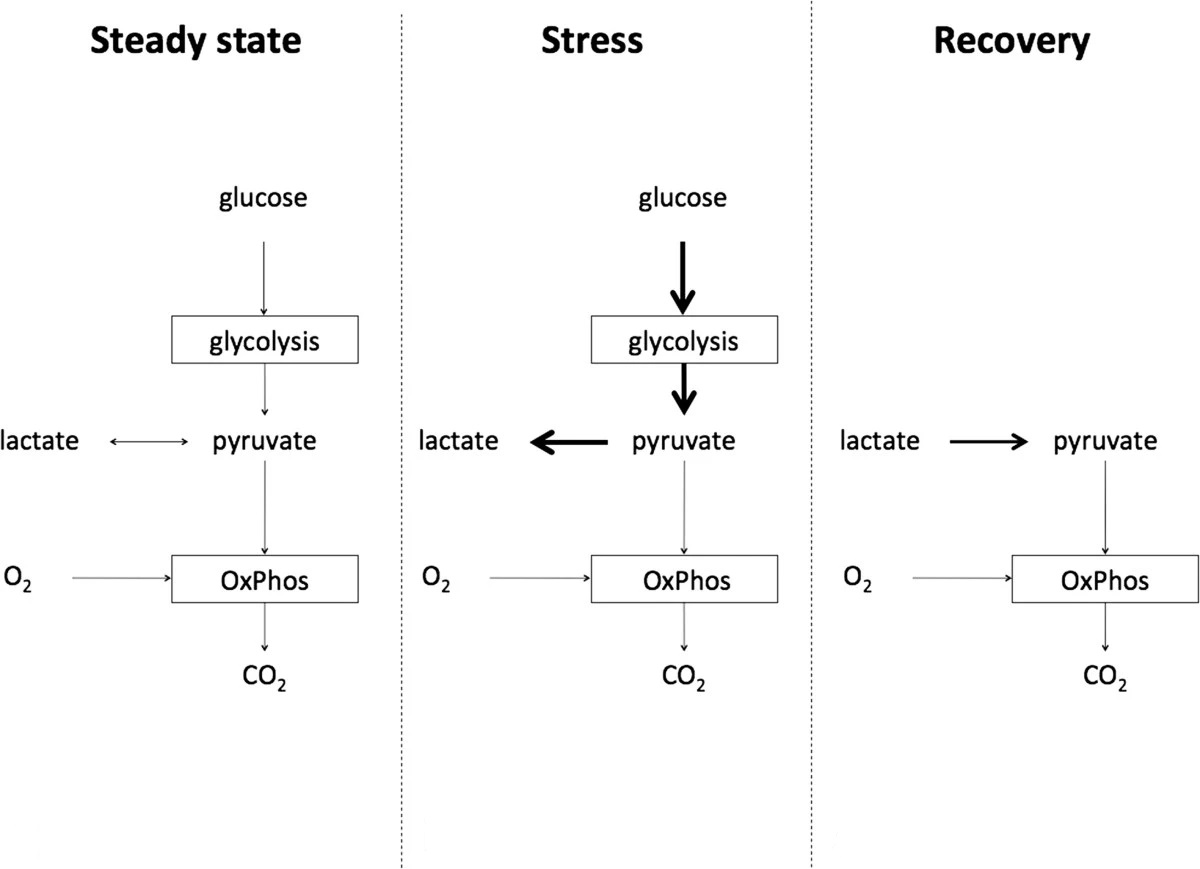
\includegraphics[width=14cm]{fig/chapter2/Cellular.jpg}
\caption{Lactate at the three different cellular levels \cite{bakker_clinical_2013}}
\label{fig:cellularlactate}
\end{figure}

{\hskip 1em} Figure \ref{fig:physiologicallactate} illustrates the association between glucose and lactate, physiologically. As it is shown, only the liver and the kidneys can reconvert lactate to pyruvate through the Cori cycle (denoted by \text{*}), which exports glucose and consumes \acrfull{ATP} (gluconeogenesis) \cite{kushimoto_lactate_2016}. This complex association of glucose and lactate brings about a hypothesis of taking both into account in identifying sicker patients. \

\begin{figure}[t]
\centering
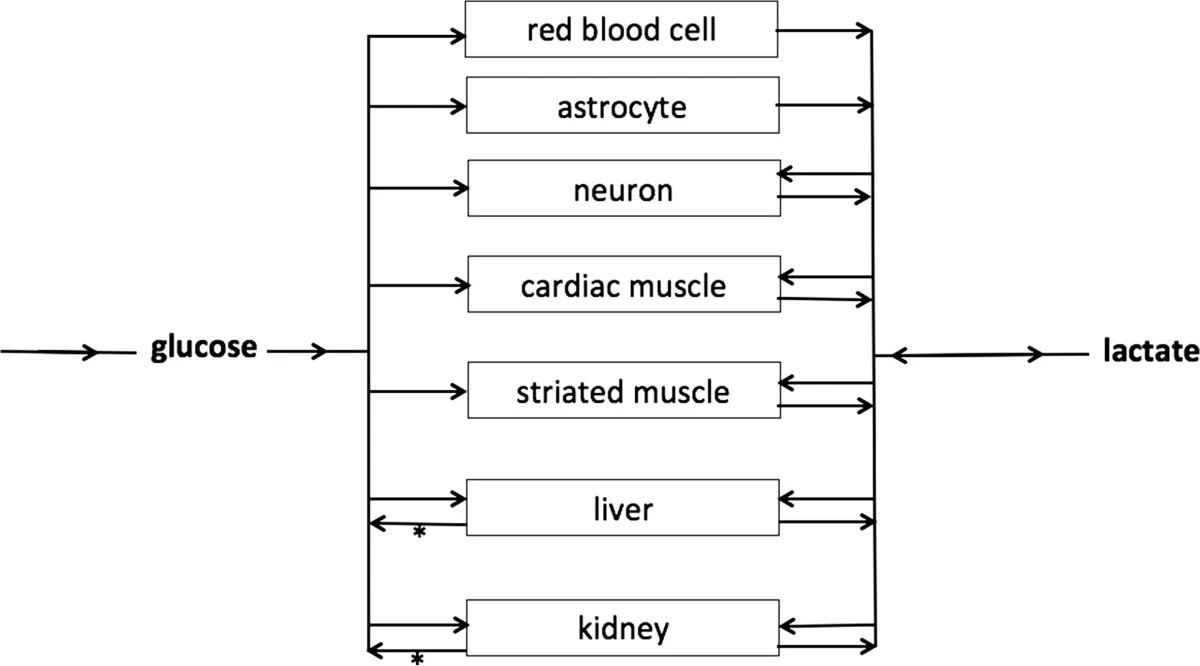
\includegraphics[width=14cm]{fig/chapter2/Physiological.jpg}
\caption{Lactate at the physiological level \cite{bakker_clinical_2013}}
\label{fig:physiologicallactate}
\end{figure}

{\hskip 1em} In \cite{sotello_glucose_nodate}, Sotello et al. argued that the glucose and lactate levels combination predicts mortality better than each value alone. Freire Jorge et al. claimed that hyperlactatemia combined with normal glucose levels is related to increased hospital mortality \cite{freire_jorge_association_2017}. Chen et al. stated that the lactate level, along with high- and low- glucose groups, is associated with in-hospital mortality. However, in the normal-glucose group, some medical scoring systems such as \acrshort{SOFA} or \acrshort{APACHE} should be utilized \cite{chen_impact_2019}. \

\section{eICU and Mortality}

The \acrlong{eICU-CRD} was published in 2019. Currently, more than 60 articles or book chapters have cited \acrshort{eICU} as their reference and are still counting ever since. Many of them focused on hospital mortality in critically ill patients. In \cite{byerly_vitamin_2020}, it is expressed that the combination of vitamin C and thiamine significantly reduces the mortality of critically ill septic patients. Deshmukh et al. \cite{deshmukh_explainable_2020} developed an \acrshort{ML} model that outperforms the \acrshort{APACHE} IVa scoring system in classifying the low-risk patients admitted with \acrfull{GI} bleed. The association of heart rate with hospital mortality in elderly and non-elderly critically ill patients was discussed in \cite{zhou_effect_2020}. Zhou et al. \cite{zhou_time_2020} studied the association of the proportion of time spent in oxygen saturation 95-99\% with reduced mortality in mechanically ventilated critically ill patients. They also surveyed the effect of age on the association of \acrfull{BMI} with in-hospital mortality \cite{zhou_obesity_2020}. Greco et al. \cite{greco_diabetes_2018} found that in non-diabetic patients, there is an association between glucose and lactate levels with glycemic variability, unlike in patients with \acrshort{DM}, where this relationship does not change by insulin remedy as the association is dramatically reduced. This study revealed that hyperlactatemia is associated with higher mortality and glucose levels along with \acrshort{DM} modifying this association in a three-way interaction.
\providecommand\phantomsection

\chapter{Dataset}\label{chap:dataset}

\section{electronic Intensive Care Unit}\label{sec:eicu}

\acrfull{eICU-CRD} Version 2.0 is an open access, multicenter critical care database published by Philips Healthcare in partnership with the MIT \acrfull{LCP}. It contains data of 200,859 ICU admissions for 139,367 unique patients in 208 hospitals across the United States. The data were employed from 2014 and 2015 \cite{cosgriff_developing_2019}, but it has been publicly available\footnote{\href{https://eicu-crd.mit.edu/}{https://eicu-crd.mit.edu/}} since April 2019. \acrshort{eICU} includes 31 tables that can be categorized into five different divisions based on types of data: \

\begin{itemize}
    \item care documentation
    \item \acrshort{APACHE}
    \item care plan
    \item administration
    \item monitor data
\end{itemize}

{\hskip 1em} An informative summary of these tables is shown in table \ref{tab:maindemo}. All tables are related to each other, except \textit{hospital}, using an identifier called {\small\fontfamily{pcr}\selectfont{patientunitstayid}}. Generally, there are three identifiers in \acrshort{eICU}:

\begin{itemize}
    \item {\small\fontfamily{pcr}\selectfont{patientunitstayid}}
    \item {\small\fontfamily{pcr}\selectfont{patienthealthsystemstayid}}
    \item {\small\fontfamily{pcr}\selectfont{uniquepid}}
\end{itemize}

{\hskip 1em} How these identifiers are related is illustrated in figure \ref{fig:eicuidentifiers}. The figure demonstrates that each {\small\fontfamily{pcr}\selectfont{patienthealthsystemstayid}} has at least one or more {\small\fontfamily{pcr}\selectfont{patientunitstayid}}, and each {\small\fontfamily{pcr}\selectfont{uniquepid}} can have multiple {\small\fontfamily{pcr}\selectfont{patienthealthsystemstayid}} or {\small\fontfamily{pcr}\selectfont{patientunitstayid}}. An example of such relations can be seen in figure \ref{fig:patienttable}, where the patient has one  {\small\fontfamily{pcr}\selectfont{uniquepid}} with two {\small\fontfamily{pcr}\selectfont{patienthealthsystemstayid}}s and four different {\small\fontfamily{pcr}\selectfont{patientunitstayid}}s.

\begin{table}[!htbp]
\centering
\setlength\tabcolsep{15pt}
\caption{\label{tab:maindemo}Summary of available measurements for the two versions of the \acrshort{eICU-CRD}}
\resizebox{0.87\textwidth}{!}{%
\begin{tabular}{@{}llll@{}}
\toprule
\thead{Table} & \thead{No. of Columns} & \thead{Demo Version Rows} & \thead{Main Version Rows} \\ \midrule \midrule
admissionDrug               & 14    & 7,417     & 874,920       \\ \midrule
admissionDx                 & 6     & 7,578     & 626,858       \\ \midrule
allergy                     & 13    & 2,475     & 251,949       \\ \midrule
apacheApsVar                & 26    & 2,205     & 171,177       \\ \midrule
apachePatientResult         & 23    & 3,676     & 297,064       \\ \midrule
apachePredVar               & 51    & 2,205     & 171,177       \\ \midrule
carePlanCareProvider        & 8     & 5,627     & 502,765       \\ \midrule
carePlanEOL                 & 5     & 15        & 1,433         \\ \midrule
carePlanGeneral             & 6     & 33,148    & 3,115,018     \\ \midrule
carePlanGoal                & 7     & 3,633     & 504,139       \\ \midrule
carePlanInfectiousDisease   & 8     & 112       & 8,056         \\ \midrule
customLab                   & 7     & 30        & 1,082         \\ \midrule
diagnosis                   & 7     & 24,978    & 2,710,672     \\ \midrule
hospital                    & 4     & 186       & 208           \\ \midrule
infusionDrug                & 9     & 38,256    & 4,803,719     \\ \midrule
intakeOutput                & 12    & 100,466   & 12,030,289    \\ \midrule
lab                         & 10    & 434,660   & 39,132,531    \\ \midrule
medication                  & 15    & 75,604    & 7,301,853     \\ \midrule
microLab                    & 7     & 342       & 16,996        \\ \midrule
note                        & 8     & 24,758    & 2,254,179     \\ \midrule
nurseAssessment             & 8     & 91,589    & 15,602,498    \\ \midrule
nurseCare                   & 8     & 42,080    & 8,311,132     \\ \midrule
nurseCharting               & 8     & 1,477,163 & 151,604,232   \\ \midrule
pastHistory                 & 8     & 12,109    & 1,149,180     \\ \midrule
patient                     & 29    & 2,520     & 200,859       \\ \midrule
physicalExam                & 6     & 84,058    & 9,212,316     \\ \midrule
respiratoryCare             & 34    & 5,436     & 865,381       \\ \midrule
respiratoryCharting         & 7     & 176,089   & 20,168,176    \\ \midrule
treatment                   & 5     & 38,290    & 3,688,745     \\ \midrule
vitalAperiodic              & 13    & 274,088   & 25,075,074    \\ \midrule
vitalPeriodic               & 19    & 1,634,960 & 146,671,642   \\ \midrule
                                                                \\
\textbf{31 Tables} & \textbf{391}  & \textbf{4,605,753} & \textbf{457,325,320} \\ \midrule
\textbf{No. of Unique Patients} &  & \textbf{1,841}     & \textbf{139,367} \\
\bottomrule
\end{tabular}}
\end{table}

\begin{figure}[ht]
\centering
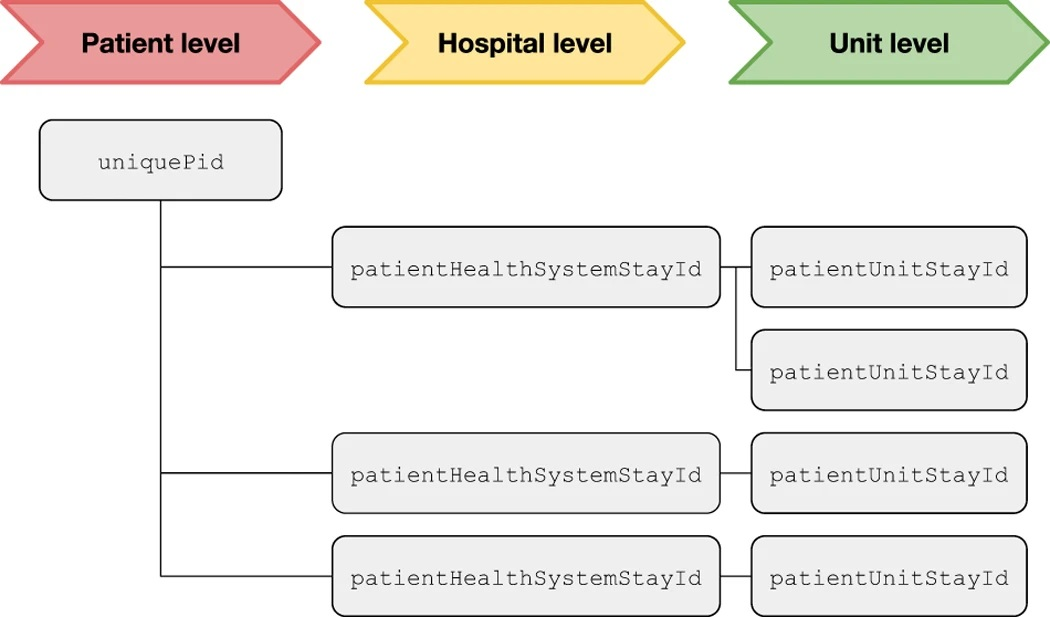
\includegraphics[width=14cm]{fig/chapter3/Organization of patient tracking information.jpg}
\caption{Organization of patient tracking information \cite{pollard_eicu_2018}}
\label{fig:eicuidentifiers}
\end{figure}

\begin{figure}[ht]
\centering
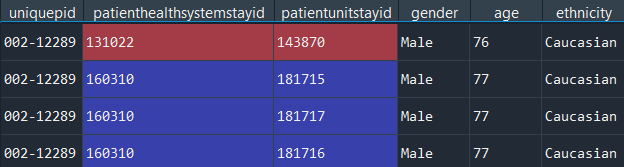
\includegraphics[width=14cm]{fig/chapter3/patient_mod.png}
\caption{Different patient identifiers in \textit{patient} table of the \acrshort{eICU-CRD}}
\label{fig:patienttable}
\end{figure}

\subsection{eICU Demo Version}

The demo version of the \acrshort{eICU} is publicly available after creating an account on the PhysioNet repository\footnote{\href{https://physionet.org/content/eicu-crd-demo/2.0/}{https://physionet.org/content/eicu-crd-demo/2.0/}}. It can be a good practice of getting to know the database, its tables, and their features before switching into the main database for our final cohort approach. In the following, the relevant tables to our goal are introduced briefly.

\subsubsection{\textit{admissionDrug}}
The table includes medication details of a patient prior to their \acrshort{ICU} admission. Since Greco et al. in \cite{greco_diabetes_2018} hypothesized that \acrshort{DM} might influence the association of hyperlactatemia with in-hospital mortality, this work is interested in separating patients who have diabetes or use drugs for glycemic control. A list of anti-diabetic medications (hereafter drug list) and their corresponding \acrshort{HICL} sequence numbers was extracted in this regard. Figure \ref{fig:admissiondrug} shows the most important parameters/columns of the \textit{admissionDrug} table for our study for a single patient. This table has the information of 449 patients (amid overall 1841 patients in the demo version of the \acrshort{eICU}), and 143 of them have the satisfying condition of the drug list.

\begin{figure}[ht]
\centering
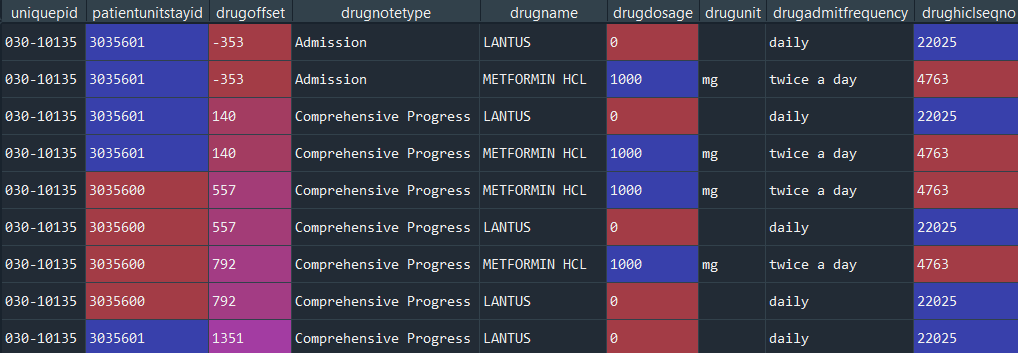
\includegraphics[width=15cm]{fig/chapter3/admissiondrug_m.png}
\caption{A slice of the \textit{admissionDrug} table for a unique patient}
\label{fig:admissiondrug}
\end{figure}

\subsubsection{\textit{admissionDx}}
This table contains the primary diagnosis for the ICU admission per the APACHE scoring criteria. This means that if a patient does not have an \textit{admissionDx} entry, they could not have an \acrshort{APACHE} score. Among 1777 patients in this table, only 145 of them were diagnosed to have a diabetic disease. Figure \ref{fig:admissiondx} shows a part of a unique patient's information in the \textit{admissionDx}.

\begin{figure}[ht]
\centering
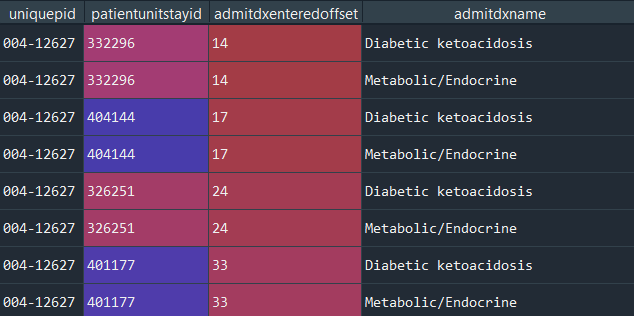
\includegraphics[width=15cm]{fig/chapter3/admissiondx_m.png}
\caption{A slice of the \textit{admissionDx} table for a unique patient}
\label{fig:admissiondx}
\end{figure}

\subsubsection{\textit{allergy}}
The \textit{allergy} table includes patients' allergies in detail. Out of 589 unique patients in this table, only ten patients have been admitted to the \acrshort{ICU} with diabetic-related allergies. A sample of the \textit{allergy} table is shown in figure \ref{fig:allergy}.

\begin{figure}[ht]
\centering
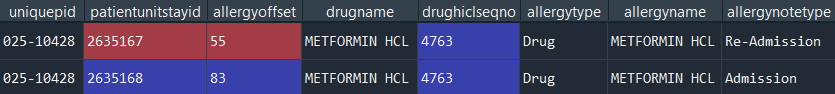
\includegraphics[width=15cm]{fig/chapter3/allergy_m.png}
\caption{A slice of the \textit{allergy} table for a unique patient}
\label{fig:allergy}
\end{figure}

\subsubsection{\textit{apacheApsVar}}
This table is the first amongst the three \acrshort{APACHE} tables in the \acrshort{eICU-CRD}. It contains the required variables for the calculation of \acrfull{APS}-III for patients in the first 24 hours of their \acrshort{ICU} admissions. The \textit{apacheApsVar} table contains information about 1786 patients, one of which can be seen in figure \ref{fig:apacheapsvar}. 

\begin{figure}[ht]
\centering
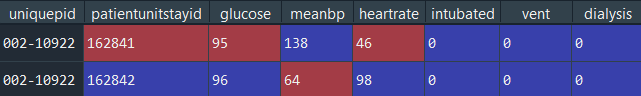
\includegraphics[width=15cm]{fig/chapter3/apacheapsvar.png}
\caption{A slice of the \textit{apacheApsVar} table for a unique patient}
\label{fig:apacheapsvar}
\end{figure}

\subsubsection{\textit{apachePatientResult}}
The \textit{apachePatientResult} table provides predictions made by the \acrshort{APACHE} score in both versions (IV and IVa) for each patient. As demonstrated in figure \ref{fig:apachepatientresult}, {\small\fontfamily{pcr}\selectfont{actualicumortality}} is a unit disposition, while {\small\fontfamily{pcr}\selectfont{actualhospitalmortality}} is a hospital disposition; each can be either EXPIRED or ALIVE. {\small\fontfamily{pcr}\selectfont{actualhospitalmortality}} is considered as the final discharge status of a patient. As of this table's provided information, there are 1512 patients out of whom 129 have the expired hospital discharge status.

\begin{figure}[ht]
\centering
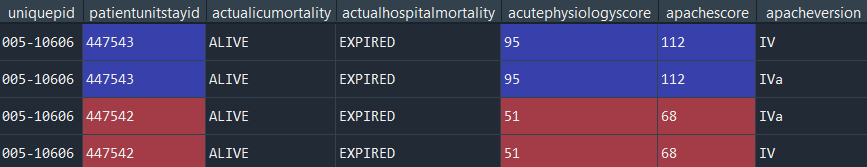
\includegraphics[width=15cm]{fig/chapter3/apachepatientresult.png}
\caption{A slice of the \textit{apachePatientResult} table for a unique patient}
\label{fig:apachepatientresult}
\end{figure}

\subsubsection{\textit{apachePredVar}}
The last \acrshort{APACHE} table provides variables underlying the APACHE predictions. In this table, {\small\fontfamily{pcr}\selectfont{gender}} 0 indicates Male, while {\small\fontfamily{pcr}\selectfont{gender}} 1 indicates Female. Furthermore, as it is seen in {\small\fontfamily{pcr}\selectfont{actualhospitalmortality}} in the \textit{apachePatientResult} table, there is a column named {\small\fontfamily{pcr}\selectfont{diedinhospital}} that is equal to the EXPIRED status in {\small\fontfamily{pcr}\selectfont{actualhospitalmortality}} when it is 1. For instance, the last row in figure \ref{fig:apachepredvar} shows that the patient with the unique patient id of 027-105179 who had diabetes, passed away one year after his (considering {\small\fontfamily{pcr}\selectfont{gender}}) admission to \acrshort{ICU}. Concerning this table, there are 369 diabetic patients, 179 EXPIRED ones, and 27 in common.

\begin{figure}[ht]
\centering
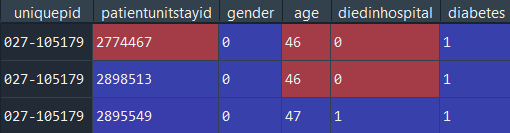
\includegraphics[width=15cm]{fig/chapter3/apachepredvar.png}
\caption{A slice of the \textit{apachePredVar} table for a unique patient}
\label{fig:apachepredvar}
\end{figure}

\subsubsection{\textit{diagnosis}}
Active patient diagnosis is recorded in the \textit{diagnosis} table, unlike the \textit{admissionDx} table with the diagnosis at admission time. There are 1709 unique patients in this table, out of whom 291 patients fulfill the drug list condition. As shown in figure \ref{fig:diagnosis}, the \textit{diagnosis} table is an explanatory one that can be used for patient stratification.

\begin{figure}[ht]
\centering
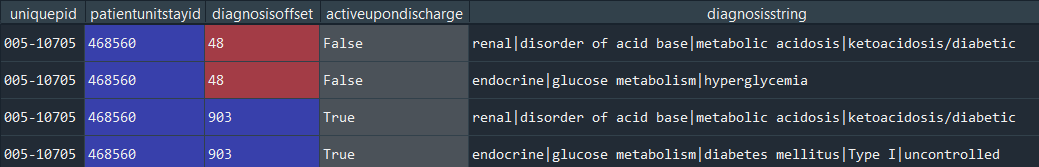
\includegraphics[width=15cm]{fig/chapter3/diagnosis_m.png}
\caption{A slice of the \textit{diagnosis} table for a unique patient}
\label{fig:diagnosis}
\end{figure}

\subsubsection{\textit{infusionDrug}}
The \textit{infusionDrug} table has the drug infusions in detail, including concentration ({\small\fontfamily{pcr}\selectfont{drugamount}}) and how the drug should be administered. It also contains {\small\fontfamily{pcr}\selectfont{patientweight}}, which is used further to complete our dataset when a weight value from the \textit{patient} table is missing. Figure \ref{fig:infusiondrug} shows part of this table.

\begin{figure}[ht]
\centering
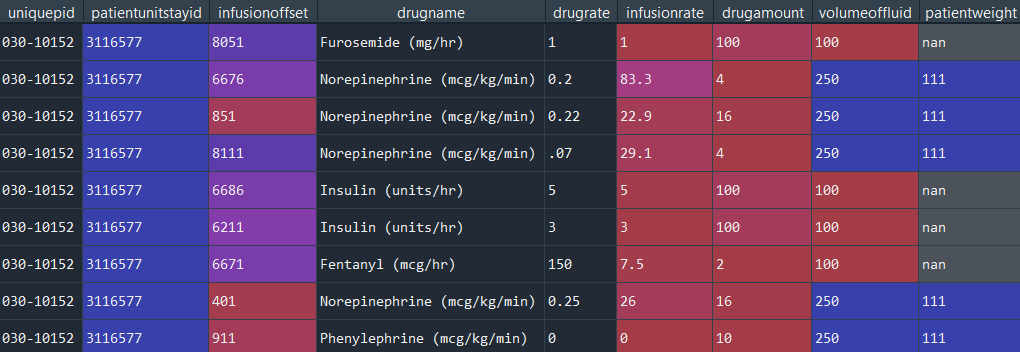
\includegraphics[width=15cm]{fig/chapter3/infusiondrug.png}
\caption{A slice of the \textit{infusionDrug} table for a unique patient}
\label{fig:infusiondrug}
\end{figure}

\subsubsection{\textit{intakeOutput}}
This table comprises of recorded intake or output of any volume for patients. For our purpose, the only record that is of interest in the \textit{intakeOutput} table (as in figure \ref{fig:intakeoutput}) is insulin, which is available for 69 patients among a total of 1633 patients in this table.

\begin{figure}[ht]
\centering
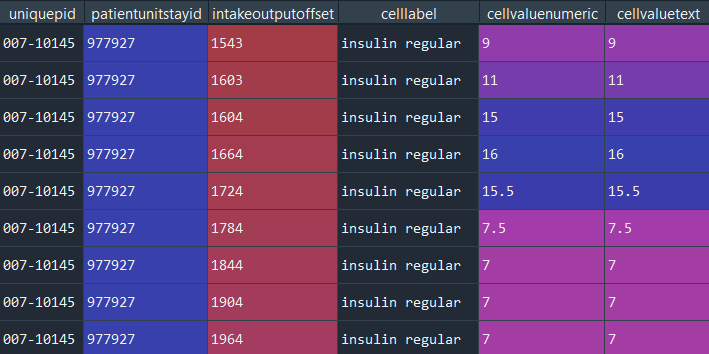
\includegraphics[width=15cm]{fig/chapter3/intakeoutput_m.png}
\caption{A slice of the \textit{intakeOutput} table for a unique patient}
\label{fig:intakeoutput}
\end{figure}

\subsubsection{\textit{lab}}
The \textit{lab} table is essential for our study. It includes all the laboratory tests for a patient collected during his/her stay in the hospital. Although there is a total of 158 distinct types of laboratory measurements \cite{pollard_eicu_2018}, regarding our objective, we are interested in just three types of measurements (see figure \ref{fig:lab}): \

\begin{itemize}
    \item glucose
    \item bedside glucose
    \item lactate
\end{itemize}

{\hskip 1em} Note that the \textit{lab} table is the only table with lactate measurement amid all the 31 tables of the \acrshort{eICU}. \

\begin{figure}[ht]
\centering
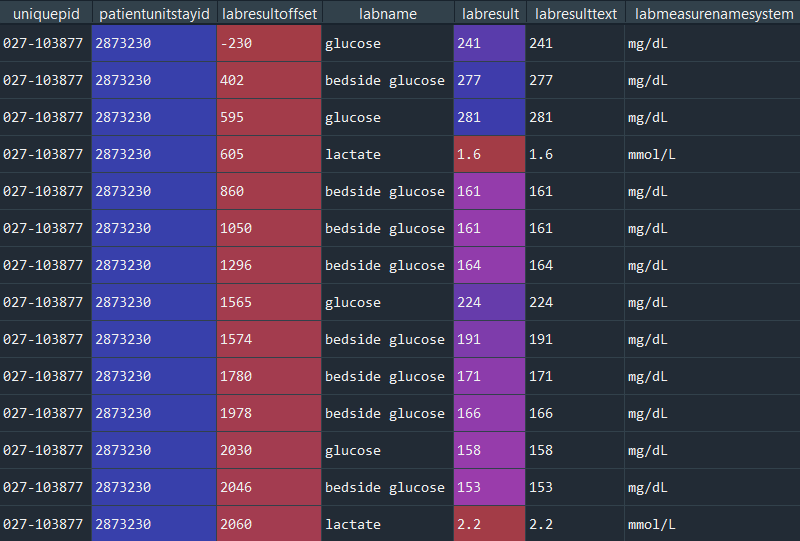
\includegraphics[width=15cm]{fig/chapter3/lab_m.png}
\caption{A slice of the \textit{lab} table for a unique patient}
\label{fig:lab}
\end{figure}

{\hskip 1em} Almost all the patients have lab measurements (1826 out of 1841), and among them, 1803 patients have at least one of the three aforementioned measurement types. The distribution of each is demonstrated in table \ref{tab:labtabledist}.

\begin{table}[h]
\centering
\setlength\tabcolsep{60pt}
\caption{\label{tab:labtabledist}Distribution of lactate and glucose measurements in the \textit{lab} table}
\begin{tabular}{@{}rc@{}}
\toprule
\thead{Measurement}            & \thead{No. of Patients} \\ \midrule \midrule
\textbf{glucose}               & 857                     \\ \midrule
\textbf{bedside glucose}       & 1245                    \\ \midrule
\textbf{lactate}               & 811                     \\
\bottomrule
\end{tabular}
\end{table}

{\hskip 1em} Since lactate is one of the crucial elements needed for our dataset, a maximum of 811 patients from the \textit{lab} table can be used should those patients have glucose measurements as well.

\subsubsection{\textit{medication}}
The \textit{medication} table consists of active medication orders for patients. However, these orders might not necessarily be administered, and the table does not provide information in this regard. The information of 1372 patients is available in this table, while 826 of them have our desired drug list expectation. Take into consideration that  {\small\fontfamily{pcr}\selectfont{\acrfull{PRN}}} is a Latin phrase that means "as needed." This indicates that it is meaningful as long as {\small\fontfamily{pcr}\selectfont{\acrshort{PRN}}} is set to YES, which is in line with the {\small\fontfamily{pcr}\selectfont{frequency}}.

\begin{figure}[ht]
\centering
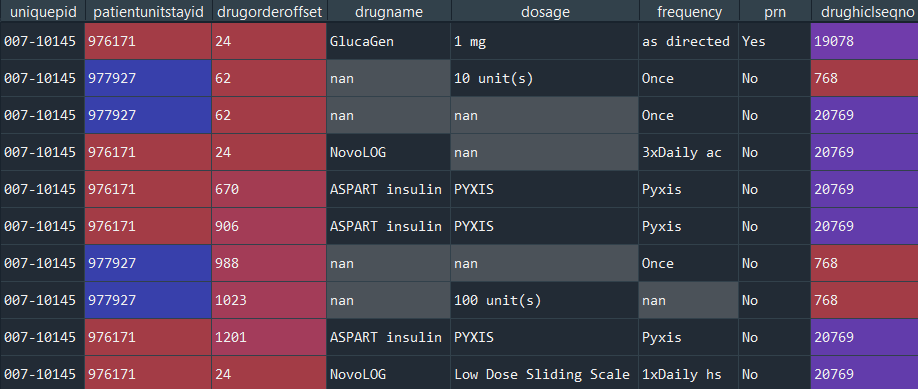
\includegraphics[width=15cm]{fig/chapter3/medication_m.png}
\caption{A slice of the \textit{medication} table for a unique patient}
\label{fig:medication}
\end{figure}

\subsubsection{\textit{nurseCharting}}
The \textit{nurseCharting} table is a nurse-entered information table in which, based on our needed values, it just has bedside glucose measurements. The number of such measurements is available for 481 out of 1786 patients. Part of this table is shown in figure \ref{fig:nursechart}.

\begin{figure}[ht]
\centering
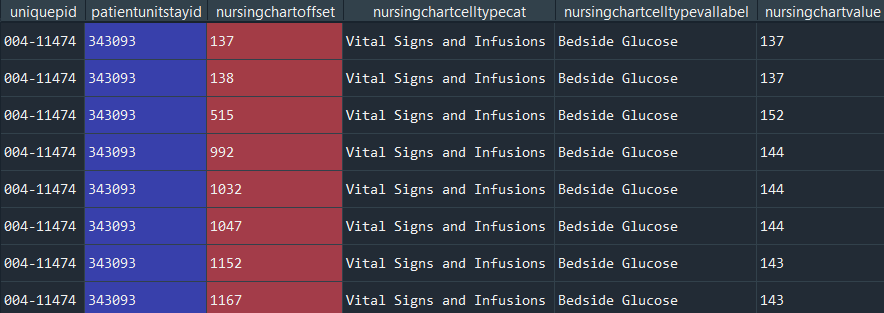
\includegraphics[width=15cm]{fig/chapter3/nursechart_m.png}
\caption{A slice of the \textit{nurseCharting} table for a unique patient}
\label{fig:nursechart}
\end{figure}

\subsubsection{\textit{pastHistory}}
All the relevant information related to the past medical history of a patient is stored in the \textit{pastHistory} table. It contains 1771 patients' information, 509 of them are of our interest, including all the 369 diabetic patients previously described in the \textit{apachePredVar} table.

\begin{figure}[H]
\begin{tabular}{@{}c@{}}
\begin{subfigure}{1\textwidth}
  \centering
  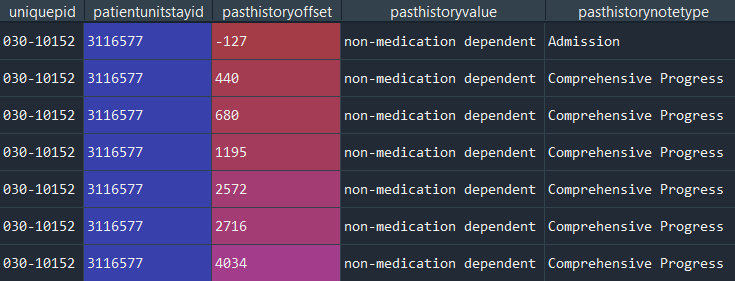
\includegraphics[width=15cm]{fig/chapter3/pasthistory_m1.png}
  \caption{\footnotesize{A patient who has diabetes type II, non-medication dependent}}
  \label{fig:pasthisotory1}
\end{subfigure} \\
\begin{subfigure}{1\textwidth}
  \centering
  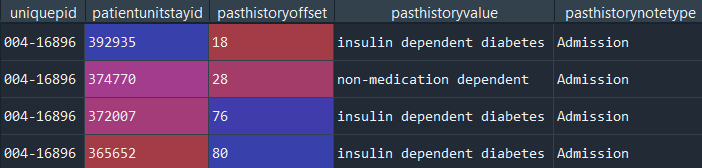
\includegraphics[width=15cm]{fig/chapter3/pasthistory_m2.png}
  \caption{\footnotesize{A patient who has diabetes type I, insulin-dependent and diabetes type II, non-medication dependent}}
  \label{fig:pasthisotory2}
\end{subfigure} \\
\begin{subfigure}{1\textwidth}
  \centering
  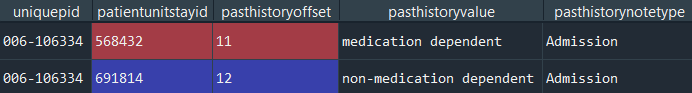
\includegraphics[width=15cm]{fig/chapter3/pasthistory_m3.png}
  \caption{\footnotesize{A patient who has diabetes type II, both medication and non-medication dependent}}
  \label{fig:pasthisotory3}
\end{subfigure} \\
\begin{subfigure}{1\textwidth}
  \centering
  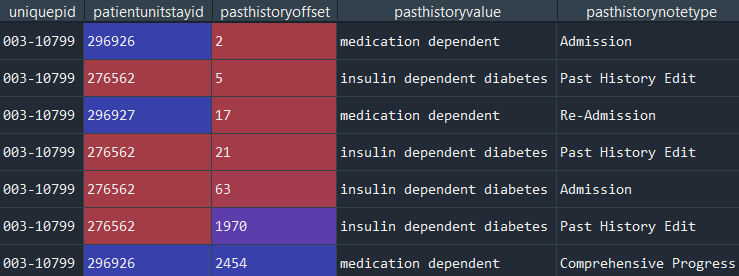
\includegraphics[width=15cm]{fig/chapter3/pasthistory_m4.png}
  \caption{\footnotesize{A patient who has diabetes type I, insulin-dependent and diabetes type II, medication dependent}}
  \label{fig:pasthisotory4}
\end{subfigure} \\
\end{tabular}
\caption{A slice of the \textit{pastHistory} table for four different diabetic patients}
\label{fig:pasthisotory}
\end{figure}

{\hskip 1em} There are two types of diabetes, diabetes type I (insulin-dependent) and diabetes type II (non-insulin-dependent), divided into two subgroups: medication dependent and non-medication dependent. As shown in figure \ref{fig:pasthisotory}, there are some intersections between these types for a unique patient. Table \ref{tab:diabeticdist} represents the distribution of the different types of diabetic patients and the number of intersections in the \textit{pastHistory} table.

\begin{table}[ht]
\centering
\setlength\tabcolsep{10pt}
\caption{\label{tab:diabeticdist}Distribution of the different types of diabetic patients}
\resizebox{0.95\textwidth}{!}{%
\begin{tabular}{@{}cccc@{}}
\toprule
\multirow{2}{*}{\thead{Diabetes}} & \thead{Type I} & \thead{Type II} & \thead{Type II} \\
& \thead{Insulin-dependent} & \thead{Medication dependent} & \thead{Non-medication dependent} \\ \midrule \midrule
\textbf{Type I}             & \multirow{2}{*}{216}    & \multirow{2}{*}{34}     & \multirow{2}{*}{3}       \\ 
\textbf{Insulin-dependent}  \\ \midrule
\textbf{Type II}                   & \multirow{2}{*}{34}     & \multirow{2}{*}{239}    & \multirow{2}{*}{6}     \\
\textbf{Medication dependent} \\ \midrule
\textbf{Type II} & \multirow{2}{*}{3} & \multirow{2}{*}{6} & \multirow{2}{*}{54}\\
\textbf{Non-medication dependent} \\
\bottomrule
\end{tabular}}
\end{table}

\subsubsection{\textit{patient}}
The \textit{patient} table includes patient demographic information and admission/discharge details during hospitalization. As discussed earlier in section \ref{sec:eicu}, all three patient identifiers were contained only in this table. The cohort selection of our work is started by patient stratification using the \textit{patient} table.

\subsubsection{\textit{treatment}}
Our study's last useful table is the \textit{treatment} table, which contains the patient's active treatments. There are 1518 patients in this table, out of whom 333 are of interest to the investigation based on the drug list. Figure \ref{fig:treatment} shows part of this table for a single patient.

\begin{figure}[ht]
\centering
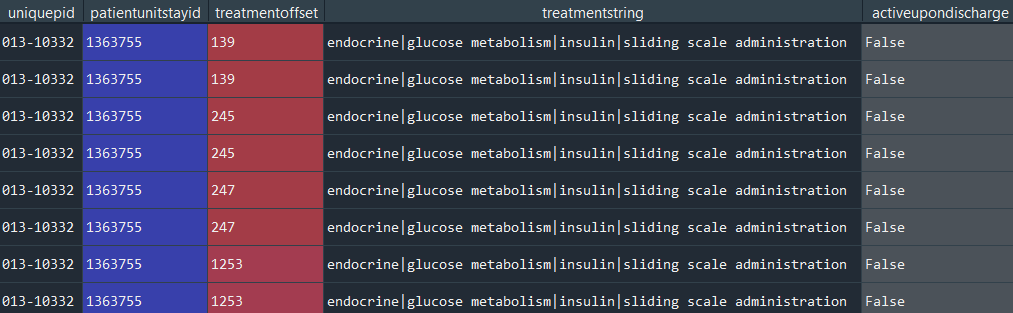
\includegraphics[width=15cm]{fig/chapter3/treatment_m.png}
\caption{A slice of the \textit{treatment} table for a unique patient}
\label{fig:treatment}
\end{figure}

\subsection{eICU Main Version}
In order to have access to the main version of the \acrshort{eICU}, one needs to complete the \acrshort{CITI} “Data or Specimens Only Research” course. Once the application completion is approved, the \acrshort{eICU-CRD} main version (Version 2.0) is accessible via PhysioNet repository\footnote{\href{https://physionet.org/content/eicu-crd/2.0/}{https://physionet.org/content/eicu-crd/2.0/}}. A brief comparison of the two versions of the \acrshort{eICU} was given in table \ref{tab:maindemo}. The main version has the exact 31 tables as in the demo version but with a factor of nearly 80 times the number of patients contained in the demo version, and hence, measurements. Having such a massive size of over 457 million rows of measurements sets some limitations in thoroughly analyzing this database as presented for its demo version using a local computer. Therefore, the \acrfull{HUNT} Cloud service was used, which had its own drawbacks. All of these limitations will be discussed in section \ref{ssec:limit}. However, the \acrshort{eICU-CRD} main version is our principal database for further analysis. 

\section{Cohort Selection}
Amongst all the 31 tables, 391 columns, and 457,325,320 rows of the \acrshort{eICU} database, we need to extract a cohort for the implementation. In this regard, first, it is necessary to select the related features to our goal. As we seek the association of glucose and lactate with mortality, both are chosen to build our dataset. Besides these two variables, we are interested in finding the importance of some demographic information, such as age, gender, and weight. Furthermore, considering the conducted survey of Greco et al. \cite{greco_diabetes_2018}, we select diabetes as one of our features to deepen our study. All in all, our ideal dataset consists of 139,367 rows (number of patients) and six columns as the following:

\begin{itemize}
    \item age
    \item gender
    \item weight
    \item glucose level
    \item lactate level
    \item diabetes
\end{itemize}

{\hskip 1em} To add more details to our study, weight is replaced by admission weight and discharge weight. Moreover, unlike the glucose level that can be found in various tables (e.g., \textit{apacheApsVar}, \textit{lab}, \textit{medication}), since the lactate level is only in the \textit{lab} table, our dataset rows are reduced to the number of patients who have a lactate value. On the other hand, having abundant glucose values and just a few lactate values for the desired patient leads us to use a standard format for each, in this case, the minimum, the mean, and the maximum level of the glucose and lactate values. Contemplating the above discussion and knowing the objective is to predict mortality, our extracted cohort has a template similar to table \ref{tab:cohorttemplate}. \

{\hskip 1em} Now that we know what features we want to include in our dataset, what matters is the number of rows to fill in the cohort. Figure \ref{fig:cohortselection} shows the steps taken to reach the final dataset. Although \acrshort{eICU-CRD} has 139,367 distinct patients, 79,768 patients have no lactate value in their records in the \textit{lab} table and must be discarded. This means only 59,599 patients remain; among those, 97 patients have \acrfull{NaN} lactate value. Thus, the number of rows diminishes to 59,502. Considering other features, it can be realized that there are 311 patients whose admission weight or discharge weight is \acrshort{NaN} as well. This dwindles the rows to 59,191. Eventually, a patient exists with age zero who must be omitted from the cohort, and that makes our dataset have 59,190 rows (patients) with 12 columns (features). The first 11 ones are input to our machine, and the last one, mortality, is used as output. 

\begin{table}[ht]
\centering
\setlength\tabcolsep{8pt}
\caption{\label{tab:cohorttemplate}Selected features for our dataset}
\resizebox{1\textwidth}{!}{%
\begin{tabular}{@{}cccccccccccc@{}}
\toprule
\multirow{2}{*}{\thead{age}} & \multirow{2}{*}{\thead{gender}} & \thead{admission} & \thead{discharge} & \thead{minimum} & \thead{mean} & \thead{maximum} & \thead{minimum} & \thead{mean} & \thead{maximum} & \multirow{2}{*}{\thead{diabetes}} & \multirow{2}{*}{\thead{mortality}} \\
    & & \thead{weight} & \thead{weight} & \thead{glucose} & \thead{glucose} & \thead{glucose} & \thead{lactate} & \thead{lactate} & \thead{lactate} \\
\bottomrule
\end{tabular}}
\end{table}

\begin{figure}[ht]
\centering
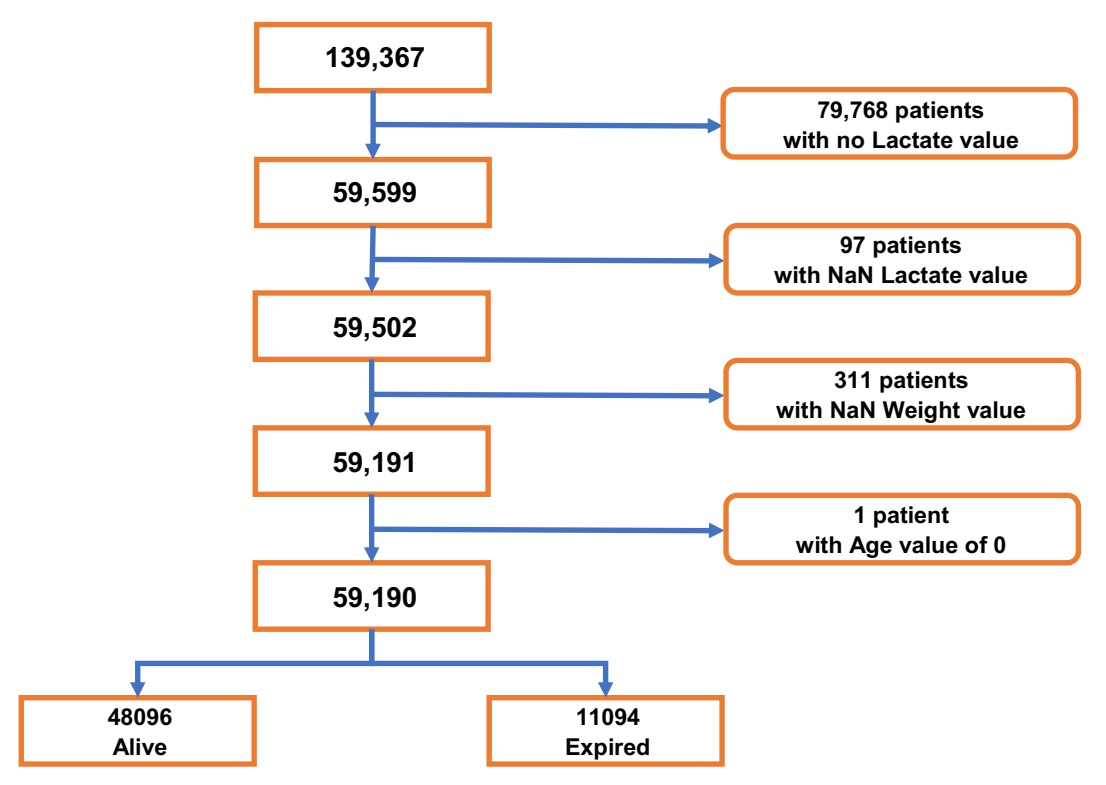
\includegraphics[width=15cm]{fig/chapter3/Cohort Selection Process.jpg}
\caption{Cohort selection process}
\label{fig:cohortselection}
\end{figure}

\subsection{Problems and Limitations}{\label{ssec:limit}}
Obtaining the final cohort was the most time-consuming step of the investigation. The challenges encountered in work are listed as follows: \

\begin{enumerate}[label=\alph*)]
    \item The \acrshort{HUNT} Cloud service was used for implementations and computations of the underway project. The \acrshort{eICU-CRD} has been merely uploaded on and accessible via the Cloud. However, working with a 2.4 GHz Intel Xeon\textregistered{} E5-2680 processor and 16 GB of memory, especially when there is a requirement to separate each patient in order not to bias the training set at the \acrlong{ML} level, could be problematic. It brought about an inability to statistically analyze the \acrshort{eICU} main version in the same manner as performed for the demo version.
    \item A patient with age "0" and some patients with age "\textgreater 89" were found in the database.
    \item For the weight value, we encountered three occasions:
    \begin{enumerate}[label=\arabic*)]
        \item there is value for admission weight, but \acrshort{NaN} for discharge weight, or vice versa.
        \item there is \acrshort{NaN} for both admission and discharge weight.
        \item either of the admission weight or discharge weight was inserted wrong regarding the unit conversion or decimal separator.
    \end{enumerate}
    \item The number of patients with lactate value(s) decreased the number of our cohort rows by more than 57\%.
    \item A patient may be discharged from \acrshort{ICU} with ALIVE status and be discharged from the hospital as EXPIRED, but the opposite is impossible. However, the \acrshort{eICU-CRD} has some of these weird cases.
\end{enumerate}

\subsection{Solutions and Assumptions}
In this section, feasible solutions for the claimed problems in section \ref{ssec:limit} are addressed one by one:

\begin{enumerate}[label=\alph*)]
    \item We focused only on the tables with our designated features. The  \textit{patient} table, the \textit{apachePredVar} table, the \textit{infusionDrug} table, and the \textit{lab} table were the only tables we took into account to create the cohort.
    \item The zero-aged patient was omitted as the information was misleading. The patients who were more than 89 years old, based on the suggestion of the \acrshort{eICU-CRD} website, were assumed to be 90-year-old patients.
    \item In regards to the problem mentioned in the previous section:
    \begin{enumerate}[label=\arabic*)]
        \item we first tried to check whether the weight information is available in the \textit{infusionDrug} table. If not, we replaced the \acrshort{NaN} value with the value of the existing one.
        \item we eliminated the whole row belonging to that specific patient. In case this was the only available weight information, the whole patient's information was disregarded.
        \item dealing with outliers is not a straightforward procedure. As a matter of fact, it is a case that should be treated patient by patient, which is cumbersome. In some cases, it was recognized that one of the values is somehow converted from "lb" to "kg" or a decimal point is missed. Nevertheless, some could be deduced by perception. For instance, a patient cannot get admitted to a hospital with 75 kg and be discharged with 209 kg!
    \end{enumerate}
    \item As described before, we have access to a patient's glucose values through different tables: \textit{apacheApsVar}, \textit{lab}, \textit{medication}, \textit{nurseCharting}, and \textit{treatment}. However, the only table that provides us with the lactate value is the \textit{lab} table. Hence, the number of studied patients for our case could not exceed that. Despite losing nearly 80,000 rows of information, the number of remaining rows is still acceptable and provides sufficient data to analyze.
    \item Mortality status is available in two tables, \textit{patient} and \textit{apachePredVar}. We must check if both tables report the same result.
\end{enumerate}

{\hskip 1em} Ultimately, after applying all the corrections for the plausible problems, should there still be any \acrshort{NaN} value in a row, the entire row would be excluded from the final dataset. \

{\hskip 1em} It is also worth mentioning that one of the features that could have been considered for the cohort was insulin dosage. However, the insulin dosage was not included because the dataset's size was already reduced due to the limitation in the number of lactate values. Instead, the study focused on \acrshort{DM} as an associated feature with glucose and lactate.

\providecommand\phantomsection

\chapter{Methodology}\label{chap:method}

\section{Tools Used}
Once the preprocessed dataset is obtained, we can enter the implementation level using \acrlong{ML} algorithms. Proceeding to this level, some tools are required that are listed as the following:

\begin{itemize}
    \item \textbf{\acrshort{HUNT} Cloud\footnote{\href{https://www.ntnu.edu/mh/huntcloud/cloud-services/hunt-compute}{https://www.ntnu.edu/mh/huntcloud/cloud-services/hunt-compute}}}: It is a Cloud computing service with Linux-based virtual machines that have varying size and memory capacity. The infrastructure is affiliated to the HUNT Research Centre, Department of Public Health and Nursing, Faculty of Medicine and Health Sciences, \acrfull{NTNU}, in Norway. 
    \item \textbf{Anaconda Spyder}: The platform for our implementations in Python. Albeit there are some other platforms such as Jupyter Lab to run our codes, since we need to have access to variables via \textsl{Variable Explorer}, Anaconda Spyder has a privilege over the other platforms.
    \item \textbf{sklearn}: Scikit-learn is a Python module that provides state-of-the-art implementations of many well-known algorithms in machine learning \cite{pedregosa_scikit-learn_2011}. It has an easy-to-use interface, and it only depends on NumPy and SciPy.
    \item \textbf{xgboost}: Unlike most of the typical \acrshort{ML} algorithms which are included in the sklearn, xgboost must be installed separately. It is an optimized gradient boosting library that solves numerous data science problems quickly and accurately.
    \item \textbf{imblearn}: Python imbalanced learning package is used on datasets where one or more of the classes has significantly less/more training samples. It employs under-sampling or over-sampling techniques to provide an equal ratio of classes.
    \item \textbf{seaborn\footnote{\href{https://seaborn.pydata.org/}{https://seaborn.pydata.org/}}}: Seaborn is a Python data visualization library. It provides a high-level interface for informative statistical graphics and drawing attractive by facilitating data visualization needs.
\end{itemize}

\section{Imbalanced Dataset}
Figure~\ref{fig:aliveexpiredratio} shows the proportion of alive patients over expired ones. It indicates that in our 59190-patient cohort (53\% male), the alive patients dominate the expired patients by a factor of 4.3. Such a significant difference between the members of a binary class affects the final prediction inasmuch as it is expected that the machine estimates most of the outcomes as alive. This prediction is correct, and in most cases, it would have high accuracy, but it could have been achieved even without having expired patients in our class. This is called the \textit{accuracy paradox} and is a common mistake since classification accuracy is the first measure for model evaluation on classification problems.

\begin{figure}[h]
\centering
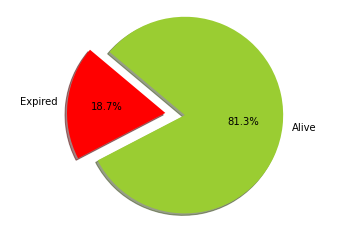
\includegraphics[width=8cm]{fig/chapter4/Alive_vs._Expired_Ratio.png}
\caption{Ratio of the Alive vs. Expired patients}
\label{fig:aliveexpiredratio}
\end{figure}

{\hskip 1em} There are techniques called resampling for balancing the number of class members before implementing the \acrlong{ML} algorithms. If samples are added to the minority class, it would be an over-sampling technique, and if samples are removed from the majority class, it would be an under-sampling technique, as depicted in figure \ref{fig:resampling}. 

\begin{figure}[h]
\centering
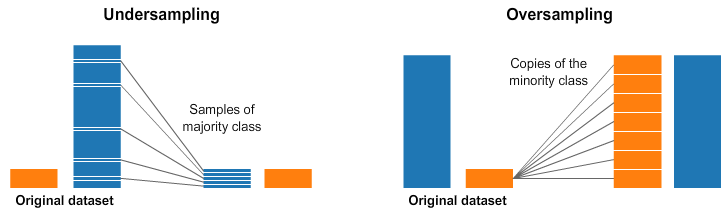
\includegraphics[width=16cm]{fig/chapter4/resampling.png}
\caption{The general concept of the resampling techniques, retrieved from \href{https://www.kaggle.com/rafjaa/resampling-strategies-for-imbalanced-datasets}{\textsl{Kaggle}}}
\label{fig:resampling}
\end{figure}

{\hskip 1em} The simplest over-sampling implementation is by duplicating random records from the minority class, bringing about overfitting. The simplest technique in under-sampling is random records removal from the majority class, giving rise to loss of information.

\subsection{Under-sampling Techniques}
Apart from random under-sampling, there are other techniques to undersample majority class, such as:

\begin{itemize}
    \item \textbf{Cluster Centroids}: It generates clustering-based centroids. Similar data should be grouped previously in order to preserve information.
    \item \textbf{Near Miss}: It comprises three versions, all of which select samples based on the distance between the majority and the minority class.
    \item \textbf{\acrlong{CNN} Rule}: \acrshort{CNN} seeks a subset of samples that leads to no loss in model performance, considered as a minimal consistent set.
    \item \textbf{Tomek Links}: It consists of removing the majority class's instances close to the minority class to space up the distance in-between; hence, facilitating the classification process.
    \item \textbf{\acrlong{ENN} Rule}: \acrshort{ENN} uses three nearest neighbors to locate misclassified samples and then uses the nearest one to make decisions.
    \item \textbf{\acrlong{OSS}}: \acrshort{OSS} is a combination of Tomek Links and \acrlong{CNN}. It involves removing the ambiguous samples on the class boundary from the majority class (Tomek Links) and then removing the redundant samples of the majority class that are far from the decision boundary (\acrshort{CNN}).
    \item \textbf{\acrlong{NCR}}: \acrshort{NCR} combines \acrshort{CNN} to remove redundant samples and \acrshort{ENN} to remove noisy or ambiguous samples.
\end{itemize}

{\hskip 1em} Concerning all the techniques mentioned above, since we lost a bunch of data due to the lactate sample limitation, we are more interested in utilizing over-sampling methods.

\subsection{Over-sampling Techniques}
There are different oversampling techniques to be applied to an imbalanced dataset. Some of their typical ones are as follows:

\begin{itemize}
    \item \textbf{Na\"ive Random Oversampling}: From the under-represented class, it generates new samples by randomly sampling with replacement of the currently available samples.
    \item \textbf{\acrlong{SMOTE}}: \acrshort{SMOTE} works by creating synthetic elements from the minor class instead of creating copies. The algorithm works by randomly selecting a point from the minority class and computing the k-nearest neighbors. The synthetic points are then added between the chosen point and its neighbors.
    \item \textbf{\acrlong{ADASYN} Sampling Method}: Derived from \acrshort{SMOTE}, \acrshort{ADASYN} has only one important difference. It biases the sample space toward the minority class.
    \item \textbf{Other Combinations}: There are other \acrshort{SMOTE}-derived techniques such as SMOTE-Boost, BorderlineSMOTE, SVMSMOTE, KMeansSMOTE, and SMOTENC that defined for particular purposes like dealing with categorical features.
\end{itemize}

{\hskip 1em} It is also possible to use an over-sampling technique followed by an under-sampling method, which yields impressive results. Whilst an over-sampling can improve the bias toward the minority class, an under-sampling can reduce the bias on the majority class. This can result in enhanced overall performance. \

{\hskip 1em} Contemplating all the aforementioned techniques and our imbalanced dataset, we chose \acrfull{SMOTE} to balance the cohort before entering the \acrlong{ML} stage. By using \acrshort{SMOTE}, as illustrated in figure \ref{fig:smote} (particularly \ref{fig:aftersmote} \& \ref{fig:balanced}), it can be seen that our dataset is balanced now and ready for further \acrshort{ML} analysis.

\begin{figure}[H]
\begin{tabular}{@{}cc@{}}
\begin{subfigure}{0.5\textwidth}
  \centering
  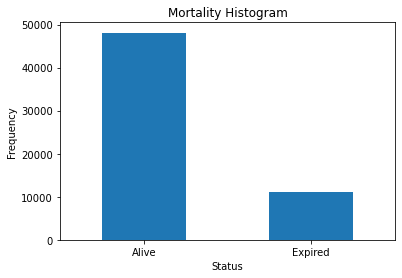
\includegraphics[width=7.5cm]{fig/chapter4/Before SMOTE.png}
  \caption{\footnotesize{Actual patients frequency}}
  \label{fig:beforesmote}
\end{subfigure} 
\begin{subfigure}{0.5\textwidth}
  \centering
  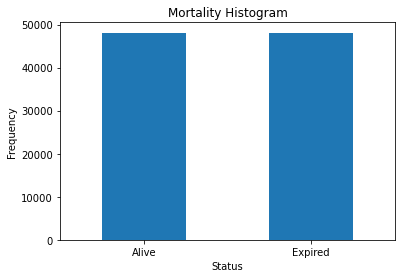
\includegraphics[width=7.5cm]{fig/chapter4/After SMOTE.png}
  \caption{\footnotesize{Patients frequency after applying \acrshort{SMOTE}}}
  \label{fig:aftersmote}
\end{subfigure} \\
\begin{subfigure}{0.5\textwidth}
  \centering
  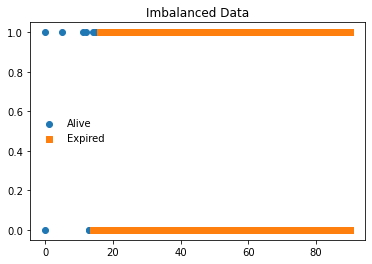
\includegraphics[width=7.5cm]{fig/chapter4/Imbalanced Data.png}
  \caption{\footnotesize{The cohort's actual scattering plot}}
  \label{fig:imbalanced}
\end{subfigure} 
\begin{subfigure}{0.5\textwidth}
  \centering
  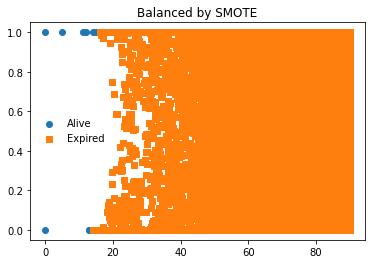
\includegraphics[width=7.5cm]{fig/chapter4/SMOTE Scattering Plot.png}
  \caption{\footnotesize{The cohort's scattering plot after applying \acrshort{SMOTE}}}
  \label{fig:balanced}
\end{subfigure} \\
\end{tabular}
\caption{Utilization of \acrshort{SMOTE} to balance an imbalanced dataset}
\label{fig:smote}
\end{figure}

\section{Glucose vs. Lactate}
Despite the fact that our primary goal is to predict mortality using various features, including glucose and lactate, it would be interesting to set a secondary goal on checking if glucose and lactate themselves are related mathematically or not. From \cite{greco_diabetes_2018}, we know that both are interdependent in carbohydrate metabolism, but as engineers, we need to find out more; perhaps, correlation can elucidate more details in this regard. Figure \ref{fig:heatmap} delineates the correlation between all the input variables of the cohort. It shows that excluding a modest association of glucose with \acrshort{DM}, which Greco et al. mentioned in \cite{greco_diabetes_2018}, there is almost no relationship between our dataset's input parameters. To make sure of this, we plotted the scattering distribution of lactate and glucose among the dataset patients based on their outcome, as shown in figure \ref{fig:gluclact}. The distribution in figures \ref{fig:gluclactmin} and \ref{fig:gluclactmean} are dense while it is widespread in figure \ref{fig:gluclactmax}. Nevertheless, in none of which, there is a clue of classification between glucose and lactate.

\begin{figure}[ht]
\centering
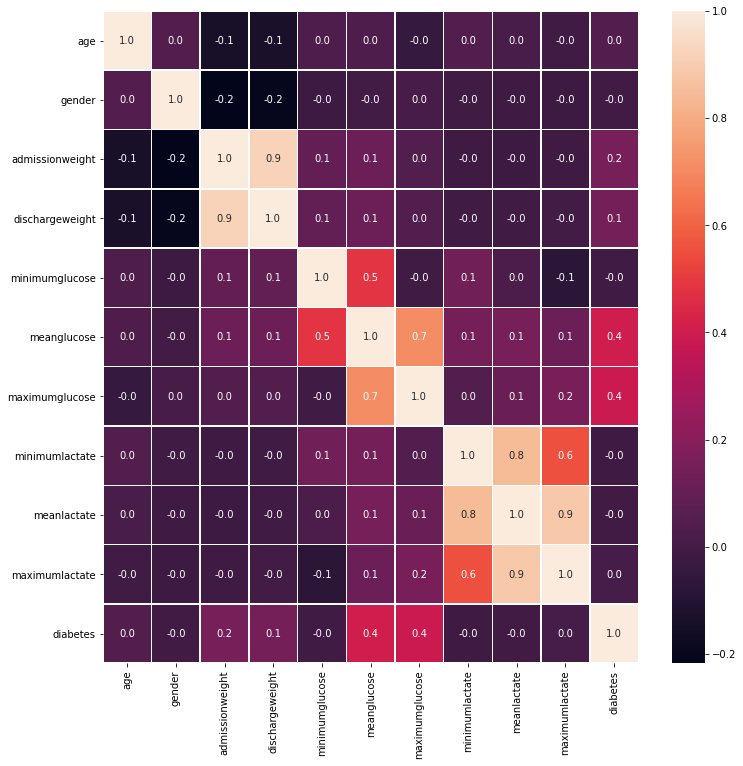
\includegraphics[width=16cm]{fig/chapter4/Heatmap.png}
\caption{The correlation matrix of the dataset}
\label{fig:heatmap}
\end{figure}

{\hskip 1em} Eventually, we take one last step and apply the pairs plot (aka scatterplot matrix) to see every variable's distribution and relationships between two variables. Looking at figure \ref{fig:pairplot}, we can rest assured that finding a mathematical relationship between glucose and lactate is way complicated.

\begin{figure}[H]
\begin{tabular}{@{}c@{}}
\begin{subfigure}{1\textwidth}
  \centering
  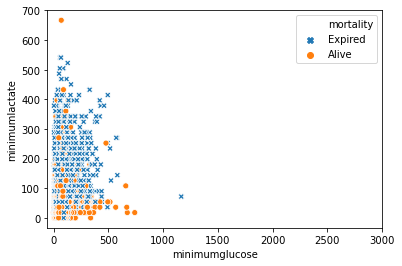
\includegraphics[width=10cm]{fig/chapter4/Glu-Lac, Min.png}
  \caption{\footnotesize{The scattering plot for the minimum values of glucose and lactate}}
  \label{fig:gluclactmin}
\end{subfigure} \\
\begin{subfigure}{1\textwidth}
  \centering
  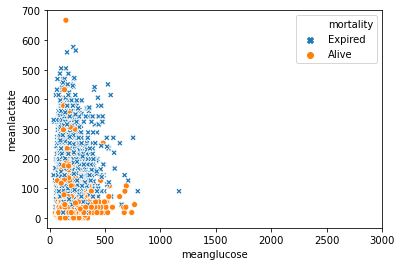
\includegraphics[width=10cm]{fig/chapter4/Glu-Lac, Mean.png}
  \caption{\footnotesize{The scattering plot for the mean values of glucose and lactate}}
  \label{fig:gluclactmean}
\end{subfigure} \\
\begin{subfigure}{1\textwidth}
  \centering
  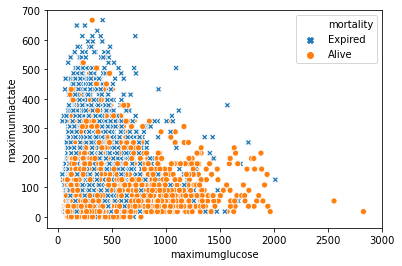
\includegraphics[width=10cm]{fig/chapter4/Glu-Lac, Max.png}
  \caption{\footnotesize{The scattering plot for the maximum values of glucose and lactate}}
  \label{fig:gluclactmax}
\end{subfigure} \\
\end{tabular}
\caption{The scattering plot of lactate vs. glucose for three different levels}
\label{fig:gluclact}
\end{figure}

\begin{figure}[ht]
\centering
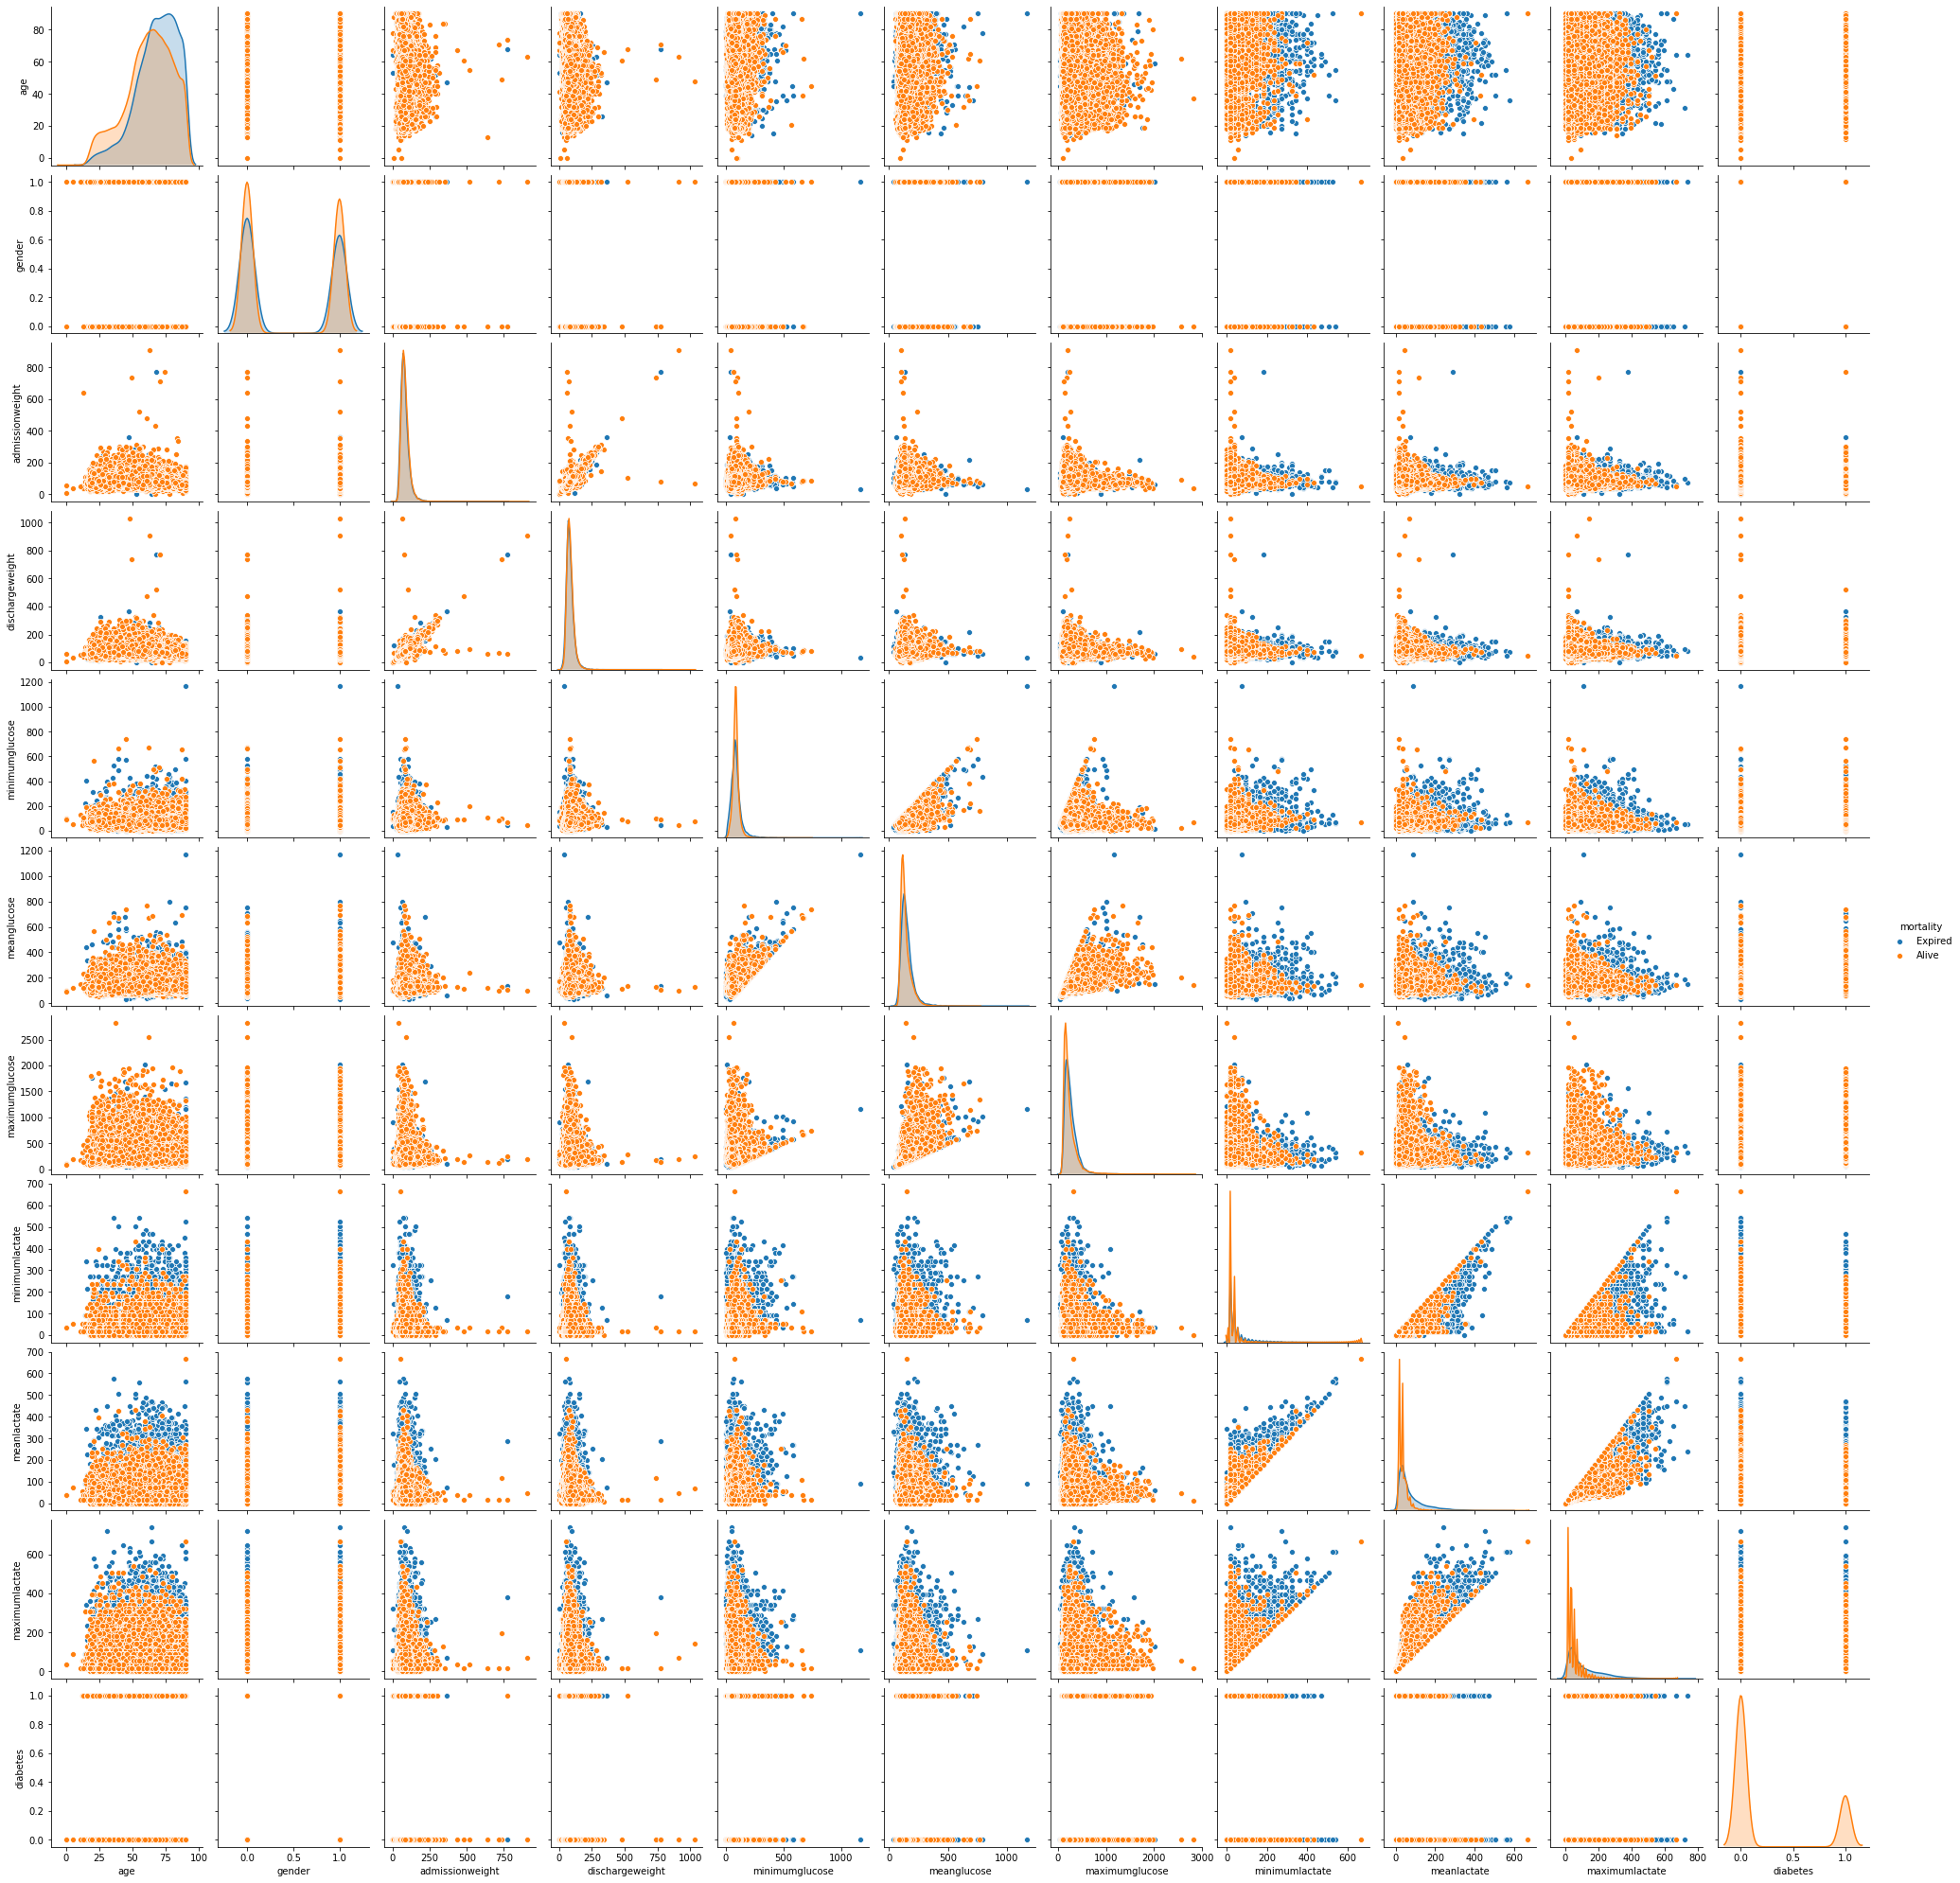
\includegraphics[width=16cm]{fig/chapter4/PairPlot.png}
\caption{The scatterplot matrix of the dataset's input features}
\label{fig:pairplot}
\end{figure}

\section{Implementation}
Seven typical linear and non-linear \acrlong{ML} algorithms have been implemented to analyze the cohort. All of them are discussed in this section. The results are given in chapter \ref{chap:results}, however. \

{\hskip 1em} Before entering the implementation level, note that 25\% of the initial cohort is split off to form a validation cohort, leaving 44,392 patients for model training if \acrshort{SMOTE} is not used and 72,144 patients if \acrshort{SMOTE} is applied. The dataset has 11 columns as input features (see figure \ref{fig:cohortselection}) and \textsl{mortality} as the binary class output feature. Moreover, the hyperparameters of all the models are selected by ten-fold cross-validation.

\subsection{Classification And Regression Tree}
Decision Tree is a supervised \acrlong{ML} algorithm used for predictive modeling. The classical \acrfull{CART} provides a basis for some useful algorithms like bagged decision trees, random forest, and boosted decision trees \cite{brownlee_master_2016}. Its representation is binary to make predictions straightforward. Each tree's root node represents an input variable, while each leaf node includes an output variable. Each new input traverses the tree starting from the root node to be evaluated. The algorithm stops splitting when a count on the number of training instances is less than a minimum threshold. \\

\begin{table}[h]
\centering
\setlength\tabcolsep{100pt}
\caption{\label{tab:carthyperparam}\acrshort{CART} basic hyperparameters}
\begin{tabular}{@{}cc@{}}
\toprule
\thead{Hyperparameter}          & \thead{Value}         \\ \midrule \midrule
Learning rate                   & 0.4                   \\ \midrule
Number of trees                 & 1                     \\ \midrule
Maximum tree depth              & 128                   \\
\bottomrule
\end{tabular}
\end{table}

{\hskip 1em} Table \ref{tab:carthyperparam} summarizes a subset of hyperparameters for the \acrshort{CART} model, while figure \ref{fig:cartfeatureimp} shows the algorithm's attributes importance. The importance default type is \textsl{gain} that indicates the average gain across all splits the feature is used in. There are also other types of feature importance, such as \textsl{weight}, \textsl{cover}, \textsl{total gain}, and \textsl{total cover}. It should be mentioned that feature importance is only defined for tree boosters.

\begin{figure}[ht]
\centering
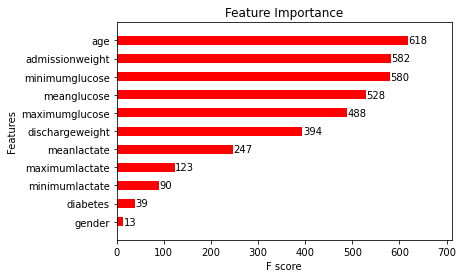
\includegraphics[width=14cm]{fig/chapter4/Feature Importance_CART.png}
\caption{\acrshort{CART} feature importance}
\label{fig:cartfeatureimp}
\end{figure}

\subsection{Extreme Gradient Boosting Decision Tree}
\acrfull{XGB} is an improved version of a Decision-Tree-based ensemble \acrlong{ML} algorithm that uses a gradient boosting framework. It is designed to enhance existing boosting techniques in the shortest amount of time by its hardware and software capabilities \cite{malik_xgboost_2020}. Unlike artificial neural networks, which are superior in unstructured data problems, for small- or medium-size tabular data problems, Decision-Tree-based algorithms are the best-in-class for now. Figure \ref{fig:xgbevolution} elaborates on the evolution of \acrshort{XGB} from Decision Trees.

\begin{figure}[ht]
\centering
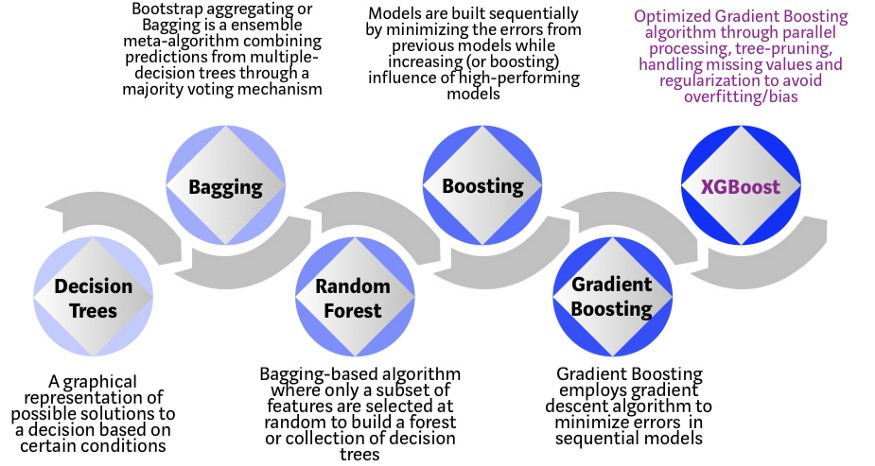
\includegraphics[width=16cm]{fig/chapter4/XGBEvolution.jpeg}
\caption{\acrshort{XGB} algorithm evolution, retrieved from \href{https://towardsdatascience.com/https-medium-com-vishalmorde-xgboost-algorithm-long-she-may-rein-edd9f99be63d}{\textsl{Towards Data Science}}}
\label{fig:xgbevolution}
\end{figure}

{\hskip 1em} Figure \ref{fig:xgbfeatures} illustrates the advantages of the \acrshort{XGB} that makes it a winning \acrlong{ML} algorithm. From parallelizing the generating trees sequential process that reduces the implementation running time to having a built-in grid search to optimize the parameters, all imply the \acrshort{XGB} is a powerful tool for our goal.

{\hskip 1em} The \acrshort{XGB} also has a built-in function to plot features ordered by their importance \cite{malik_xgboost_2020}, the same as in \acrshort{CART}. Figure \ref{fig:xgbfeatureimportance} represents the most important input features for our \acrshort{XGB} algorithm in decreasing order. Furthermore, table \ref{tab:xgbhyperparam} describes the basic hyperparameters used in our implementation.

{\hskip 1em} There is a relationship between the \textsl{Number of trees} and the depth of each tree in table \ref{tab:xgbhyperparam}. We expect that the deeper the trees are, the fewer trees are required in the model, and vice versa. That is to say, the simpler trees need more trees to achieve similar results.


\begin{figure}[ht]
\centering
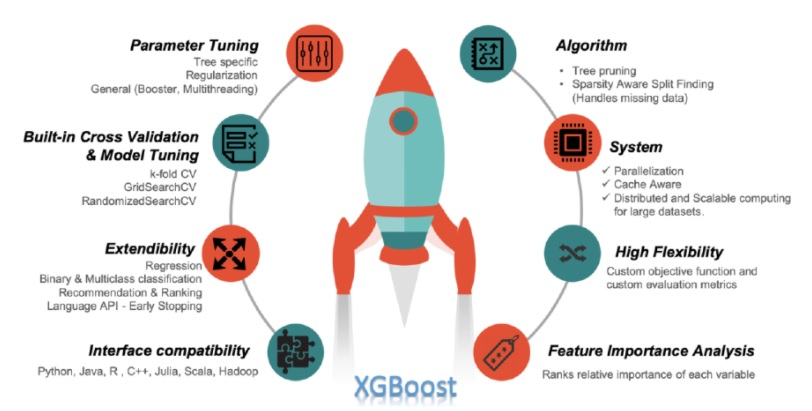
\includegraphics[width=12.7cm]{fig/chapter4/XGB Features.jpg}
\caption{\acrshort{XGB} features \cite{malik_xgboost_2020}}
\label{fig:xgbfeatures}
\end{figure}

\begin{table}[H]
\centering
\setlength\tabcolsep{100pt}
\caption{\label{tab:xgbhyperparam}\acrshort{XGB} basic hyperparameters}
\begin{tabular}{@{}cc@{}}
\toprule
\thead{Hyperparameter}          & \thead{Value}         \\ \midrule \midrule
Learning rate                   & 0.2                   \\ \midrule
Number of trees                 & 100                   \\ \midrule
Maximum tree depth              & 64                    \\
\bottomrule
\end{tabular}
\end{table}

\begin{figure}[H]
\centering
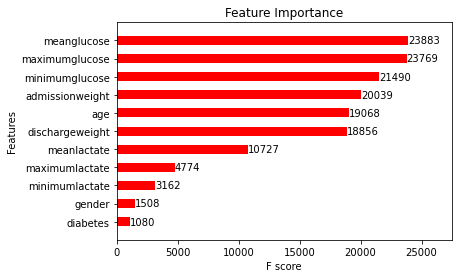
\includegraphics[width=14cm]{fig/chapter4/Feature Importance_XGB.png}
\caption{\acrshort{XGB} feature importance}
\label{fig:xgbfeatureimportance}
\end{figure}

\subsection{Support Vector Machine}
The \acrfull{SVM} algorithm finds a hyperplane decision boundary in an N-dimensional (N-feature) space that best classifies the data points into two classes. This hyperplane should have the maximum distance between the data points of both classes. Support vectors are data points closer to the hyperplane and influence the position and orientation of it.

{\hskip 1em} The \acrlong{SVM} algorithm is mostly effective for balanced datasets and binary classification. For our imbalanced cohort, \acrshort{SVM} should weigh the margin proportional to the class importance, which is often referred to as weighted \acrshort{SVM}, or cost-sensitive \acrshort{SVM} \cite{brownlee_master_2016}. The reason why we choose \textsl{Class weight} parameter as BALANCED, as shown in Table \ref{tab:svmhyperparam}, is due to using \acrshort{SMOTE} beforehand to level the two classes. Furthermore, keep in mind that setting \textsl{Probability} to TRUE slows down the method since it uses five-fold cross-validation\footnote{\href{https://scikit-learn.org/stable/modules/generated/sklearn.svm.SVC.html}{https://scikit-learn.org/stable/modules/generated/sklearn.svm.SVC.html}} internally.

\begin{table}[H]
\centering
\setlength\tabcolsep{100pt}
\caption{\label{tab:svmhyperparam}\acrshort{SVM} basic hyperparameters}
\begin{tabular}{@{}cc@{}}
\toprule
\thead{Hyperparameter}     & \thead{Value}           \\ \midrule \midrule
Kernel                     & radial basis function   \\ \midrule
Gamma                      & scale                   \\ \midrule
Class weight               & balanced                \\ \midrule
Probability                & true                    \\
\bottomrule
\end{tabular}
\end{table}

\subsection{Logistic Regression}
Like \acrshort{SVM}, \acrfull{LR} works well on binary classification, but it is not effective at imbalanced classification. \acrshort{LR} uses an optimization algorithm to minimize the negative-log likelihood (loss) on the training set. Regardless of \acrshort{SMOTE} that we used in our implementation, it is feasible to modify the loss calculation by weighing each class's importance to take the balance into consideration. This can be done by penalizing the model less/more for errors made on majority/minority class samples. This is referred to as Weighted Logistic Regression, Class-Weighted Logistic Regression, or Cost-Sensitive Logistic Regression \cite{brownlee_master_2016}. 

\begin{table}[H]
\centering
\setlength\tabcolsep{100pt}
\caption{\label{tab:lrhyperparam}\acrlong{LR} basic hyperparameters}
\begin{tabular}{@{}cc@{}}
\toprule
\thead{Hyperparameter}     & \thead{Value}           \\ \midrule \midrule
Solver                     & Newton                  \\ \midrule
Penalty                    & L2                      \\ \midrule
Class weight               & balanced                \\
\bottomrule
\end{tabular}
\end{table}

{\hskip 1em} Table \ref{tab:lrhyperparam} shows some of the basic hyperparameters used in our implementation. NEWTON's method is chosen as the model \textsl{Solver} since it uses a better quadratic function minimization. However, the LIBLINEAR method could also be used. Moreover, our algorithm's regularization technique is Ridge Regression (L2), which adds “squared magnitude” of coefficient as a penalty term to the loss function\footnote{\href{https://towardsdatascience.com/l1-and-l2-regularization-methods-ce25e7fc831c}{https://towardsdatascience.com/l1-and-l2-regularization-methods-ce25e7fc831c}}. Finally, applying \acrshort{SMOTE} makes us select the \textsl{Class weight} as BALANCED, the same as in \acrshort{SVM}.

\subsection{Na\"ive Bayes}
The Bayes Theorem assumes each input variable is dependent upon other variables. This brings about calculation complexity. By assuming independence between the variables, the calculation is simplified dramatically. This simplification is widely used for classification problems of predictive modeling and is referred to as \acrfull{NB} \cite{brownlee_master_2016}. 

There are three common distributions in the \acrlong{NB} implementation:

\begin{itemize}
    \item Bernoulli distribution
    \item Gaussian distribution
    \item Multinomial distribution
\end{itemize}

{\hskip 1em} Each of them has its own \acrlong{NB} algorithm. For our case, it is possible to use either Bernoulli \acrlong{NB} or Gaussian \acrlong{NB} algorithm. We go for the latter one, considering the parameter \textsl{priors} should be set appropriately for our imbalanced dataset.

\subsection{Linear Discriminant Analysis}
Limitations such as having a problem with multi-class classification, instability with well-separated classes, and instability with few examples diminish the \acrlong{LR} efficacy in classification problems. Nonetheless, a good alternative is using \acrfull{LDA}. 

{\hskip 1em} Making predictions in \acrshort{LDA} is preceded by computing the statistical properties of the data. It means for a single input variable, the mean and the variance of each class should be extracted, while for multiple variables, this should be done for the means and the covariance matrix \cite{brownlee_master_2016}. Afterwards, Bayes Theorem is used to estimate the probabilities in order to make predictions. 

{\hskip 1em} Table \ref{tab:ldahyperparam} represents the basic parameters used in our project's \acrshort{LDA} algorithm implementation. As can be seen, the \textsl{Solver} is chosen as \acrfull{SVD} with the chance of computing the weighted covariance matrix. The \textsl{Priors} is set to 0.5 for each class, and the \textsl{Number of components} is ONE since it must be the minimum of the number of features or the number of classes subtracted by one\footnote{\href{https://scikit-learn.org/stable/modules/generated/sklearn.discriminant_analysis.LinearDiscriminantAnalysis.html}{https://scikit-learn.org/stable/modules/generated/sklearn.discriminant\_analysis.LinearDiscriminantAnalysis}}. 

\begin{table}[H]
\centering
\setlength\tabcolsep{100pt}
\caption{\label{tab:ldahyperparam}\acrshort{LDA} basic hyperparameters}
\begin{tabular}{@{}cc@{}}
\toprule
\thead{Hyperparameter}     & \thead{Value}           \\ \midrule \midrule
Solver                     & svd                     \\ \midrule
Store covariance           & true                    \\ \midrule
Priors                     & 0.5                     \\ \midrule
Number of components       & 1                       \\
\bottomrule
\end{tabular}
\end{table}

\subsection{K-Nearest Neighbors}
\acrfull{KNN} directly uses the training set to make predictions by searching through it for the K most similar instances and summarizing the output variable, the most common class value, for them. In this regard, a distance measure (e.g., Euclidean distance, Hamming distance, Manhattan distance, Minkowski distance) should be used.

{\hskip 1em} \acrshort{KNN} is well-suited for a small number of input variables. However, for considerably large input variables, it suffers from "Curse of Dimensionality." Therefore, \acrshort{KNN} works fine if the data is low-dimensional, rescaled, and missed data is addressed \cite{brownlee_master_2016}.

{\hskip 1em} In table \ref{tab:knnhyperparam}, some basic parameters for \acrshort{KNN} model implementation are shown. Taking the \textsl{Number of neighbors} as 25, and the \textsl{Metric} as EUCLIDEAN distance gives our study the most accurate result. Besides, the \textsl{Power parameter} is set to 2 (L2), which corresponds to the selected metric.

{\hskip 1em} Apart from built-in feature importance (previously seen in \acrshort{CART} and \acrshort{XGB} sections) and SHAP model-agnostic feature importance (based on the Shapley values from game theory), there is also permutation-based feature importance that shuffles the features and calculates the change in the performance of the model\footnote{\href{https://mljar.com/blog/feature-importance-xgboost/}{https://mljar.com/blog/feature-importance-xgboost/}}. Using this method, we can see the most important features of the \acrshort{KNN}, as depicted in figure \ref{fig:knnfeatureimportance}.

\begin{table}[H]
\centering
\setlength\tabcolsep{100pt}
\caption{\label{tab:knnhyperparam}\acrlong{KNN} basic hyperparameters}
\begin{tabular}{@{}cc@{}}
\toprule
\thead{Hyperparameter}     & \thead{Value}          \\ \midrule \midrule
Number of neighbors        & 25                     \\ \midrule
Algorithm                  & auto                   \\ \midrule
Metric                     & Euclidean              \\ \midrule
Power parameter            & 2                      \\
\bottomrule
\end{tabular}
\end{table}

\begin{figure}[H]
\centering
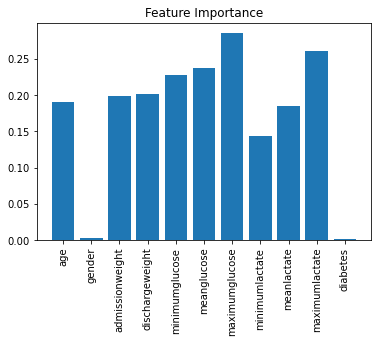
\includegraphics[width=11cm]{fig/chapter4/Feature Importance_KNN.png}
\caption{\acrlong{KNN} feature importance}
\label{fig:knnfeatureimportance}
\end{figure}
\providecommand\phantomsection

\chapter{Results}\label{chap:results}
In this chapter, the results of implementing \acrlong{ML} algorithms, discussed in chapter \ref{chap:method} are given, followed by a comparison of their performance and computational complexity.

The upcoming results were achieved under the following conditions:

\begin{itemize}
    \item The test set comprises 25\% of the initial dataset.
    \item \acrlong{SMOTE} is used to balance the skewed distribution.
    \item A 5-fold cross-validation with three repetitions is used to assess our method. Hence, the average of 15 test results is used to evaluate the effect of various methods' classification.
    \item Six criteria are used to evaluate each model: \acrlong{AUC}, Accuracy, Precision, Recall, F1-score, and Cohen's Kappa.
\end{itemize}

{\hskip 1em} Additionally, there are four more statistics obtained from each experiment and these form the Confusion Matrix. These parameters are used to calculate the metrics mentioned above (excluding Cohen's Kappa), as presented in \crefrange{eq:accu}{eq:f1sc}:

\begin{table}[H]
% \centering
\setlength\tabcolsep{5pt}
\begin{tabular}{@{}ll@{}}
\textbf{\textit{True Positive (TP):}}  & the patient is alive at the discharge time, and the prediction is \textsc{Alive}.              \\ 
\textbf{\textit{True Negative (TN):}}  & the patient died in hospital, and the prediction is \textsc{Expired}.                    \\ 
\textbf{\textit{False Positive (FP):}} & the patient is alive at the discharge time, but the prediction is \textsc{Expired}. \\ 
\textbf{\textit{False Negative (FN):}} & the patient died in hospital while the prediction is \textsc{Alive}.                      \\
\end{tabular}
\label{tab:confusionmatparam}
\vspace{-3mm}
\end{table}

{\hskip 1em} Classification accuracy, \cref{eq:accu}, is the ability of classifiers to make accurate predictions. To calculate \acrfull{ROC}, sensitivity, \cref{eq:sens}, and specificity, \cref{eq:spec}, must be obtained to draw \acrfull{AUC} for each model. In the \acrshort{ROC} curve, the horizontal axis is \textit{FPR}, and the vertical axis is \textit{TPR}. Hence, the closer the distance of the point on the \acrshort{ROC} curve to (0, 1), the
higher the classifier's accuracy \cite{ma_gradient_2019}. When instances are balanced between each class, using the \acrshort{ROC} curve is the right choice. On the contrary, the \textsc{Precision-Recall} curve is appropriate for imbalanced datasets.

{\hskip 1em} \textit{F1-score}, \cref{eq:f1sc}, computes the harmonic mean of the \textit{Precision} and \textit{Recall}. For a specific probability threshold (e.g., 0.5), \textit{F1-score} summarizes model skill, whereas the \acrlong{AUC} summarizes the skill of a model across thresholds \cite{brownlee_master_2016}.

\begin{align}
    Accuracy \ & = \ \frac{TP + TN}{TP + TN + FP + FN} \label{eq:accu} \\[10pt] 
    Sensitivity \ or \ TPR \ & = \ \frac{TP}{TP + FN}  \label{eq:sens} \\[10pt]
    Specificity \ or \ FPR \ & = \ \frac{FP}{FP + TN}  \label{eq:spec} \\[10pt]
    Precision \ & = \ \frac{TP}{TP + FP}               \label{eq:prec} \\[10pt]
    Recall \ & = \ \frac{TP}{TP + FN}                  \label{eq:recl} \\[10pt]
    F1-score \ & = \ \frac{2 \times Precision \times Recall}{Precision + Recall} \label{eq:f1sc}
\end{align} 

\smallskip
{\hskip 1em} \cref{fig:cartconfusionmat,fig:xgbconfusionmat,fig:svmconfusionmat,fig:lrconfusionmat,fig:nbconfusionmat,fig:ldaconfusionmat,fig:knnconfusionmat} show the Confusion Matrices obtained from the four pre-discussed parameters, \textit{TP}, \textit{TN}, \textit{FP}, and \textit{FN}, for all the implemented algorithms. The more the predictions fall on the matrix's diagonal line, the better the performance of our model is. \

{\hskip 1em} \crefrange{tab:cartreport}{tab:knnreport} provide detailed information about the usage of \cref{eq:accu,eq:prec,eq:recl,eq:f1sc} in our chosen models for each class. \

{\hskip 1em} The \acrshort{ROC} curve of each algorithm is shown in \cref{fig:cartroc,fig:xgbroc,fig:svmroc,fig:lrroc,fig:nbroc,fig:ldaroc,fig:knnroc}, while their respective \textsc{Precision-Recall} curve is depicted in \cref{fig:cartprerec,fig:xgbprerec,fig:svmprerec,fig:lrprerec,fig:nbprerec,fig:ldaprerec,fig:knnprerec}. As it can also be seen in \crefrange{eq:prec}{eq:recl}, \textsc{Precision-Recall} curves do not consider \textit{TN}.\

{\hskip 1em} All the corresponding developed codes that brought about this chapter's results can be found in the author's profile on GitHub repository\footnote{\href{https://github.com/mani0098/GlucoseLactateMortality}{https://github.com/mani0098/GlucoseLactateMortality}}.

\clearpage
\section{Implemented CART Results}

\begin{table}[h]
\fontfamily{pcr}\selectfont
\centering
\setlength\tabcolsep{10pt}
\caption{\label{tab:cartreport}The classification report of the \acrshort{CART} algorithm}
\resizebox{0.7\textwidth}{!}{%
\begin{tabular}{@{}rrrrr@{}}
\thead{} & \thead{precision} & \thead{recall} & \thead{f1-score} & \thead{support} \\ [12pt]
Alive         & 0.83  & 0.87  & 0.85  & 12058       \\ 
Expired       & 0.86  & 0.82  & 0.84  & 11990       \\ 
                                                    \\
accuracy      &       &       & 0.84  & 24048       \\ 
micro avg     & 0.84  & 0.84  & 0.84  & 24048       \\
weighted avg  & 0.84  & 0.84  & 0.84  & 24048       \\
\end{tabular}}
\end{table}

\begin{figure}[H]
\centering
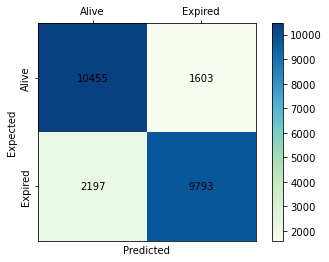
\includegraphics[width=8cm]{fig/chapter5/CART/Confusion Matrix_new.png}
\caption{Confusion matrix for the \acrshort{CART} algorithm}
\label{fig:cartconfusionmat}
\end{figure}

\begin{figure}[H]
\begin{tabular}{@{}cc@{}}
\begin{subfigure}{0.5\textwidth}
  \centering
  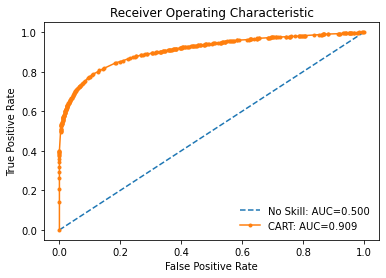
\includegraphics[width=7.5cm]{fig/chapter5/CART/ROC_new.png}
  \caption{\footnotesize{The \acrshort{ROC} curve}}
  \label{fig:cartroc}
\end{subfigure} 
\begin{subfigure}{0.5\textwidth}
  \centering
  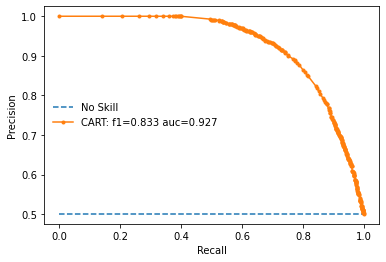
\includegraphics[width=7.5cm]{fig/chapter5/CART/Precision-Recall_new.png}
  \caption{\footnotesize{The Precision-Recall curve}}
  \label{fig:cartprerec}
\end{subfigure} \\
\end{tabular}
\caption{Curves of \acrshort{ROC} and Precision-Recall using the \acrshort{CART} algorithm}
\label{fig:cartcurves}
\end{figure}

\section{Implemented XGBoost Results}

\begin{table}[h]
\fontfamily{pcr}\selectfont
\centering
\setlength\tabcolsep{10pt}
\caption{\label{tab:xgbreport}The classification report of the \acrshort{XGB} algorithm}
\resizebox{0.7\textwidth}{!}{%
\begin{tabular}{@{}rrrrr@{}}
\thead{} & \thead{precision} & \thead{recall} & \thead{f1-score} & \thead{support} \\ [12pt]
Alive         & 0.88  & 0.94  & 0.91  & 12069       \\ 
Expired       & 0.93  & 0.87  & 0.90  & 11979       \\ 
                                                    \\
accuracy      &       &       & 0.90  & 24048       \\ 
micro avg     & 0.90  & 0.90  & 0.90  & 24048       \\
weighted avg  & 0.90  & 0.90  & 0.90  & 24048       \\
\end{tabular}}
\end{table}

\begin{figure}[H]
\centering
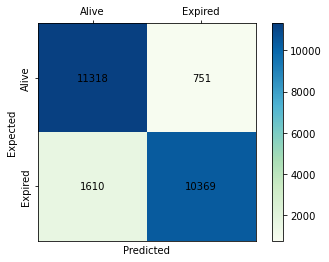
\includegraphics[width=8cm]{fig/chapter5/XGB/Confusion_Matrix_new.png}
\caption{Confusion matrix for the \acrshort{XGB} algorithm}
\label{fig:xgbconfusionmat}
\end{figure}

\begin{figure}[H]
\begin{tabular}{@{}cc@{}}
\begin{subfigure}{0.5\textwidth}
  \centering
  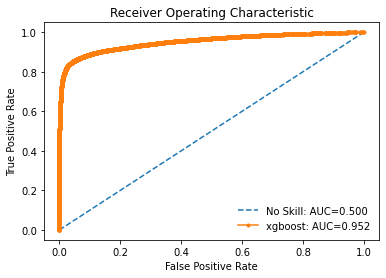
\includegraphics[width=7.5cm]{fig/chapter5/XGB/ROC_new.png}
  \caption{\footnotesize{The \acrshort{ROC} curve}}
  \label{fig:xgbroc}
\end{subfigure} 
\begin{subfigure}{0.5\textwidth}
  \centering
  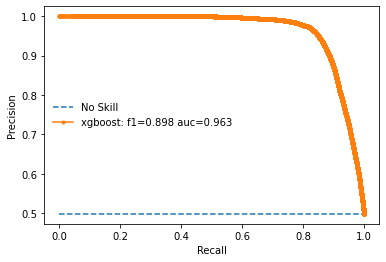
\includegraphics[width=7.5cm]{fig/chapter5/XGB/Precision-Recall_new.png}
  \caption{\footnotesize{The Precision-Recall curve}}
  \label{fig:xgbprerec}
\end{subfigure} \\
\end{tabular}
\caption{Curves of \acrshort{ROC} and Precision-Recall using the \acrshort{XGB} algorithm}
\label{fig:xgbcurves}
\end{figure}

\section{Implemented SVM Results}

\begin{table}[h]
\fontfamily{pcr}\selectfont
\centering
\setlength\tabcolsep{10pt}
\caption{\label{tab:svmreport}The classification report of the \acrshort{SVM} algorithm}
\resizebox{0.7\textwidth}{!}{%
\begin{tabular}{@{}rrrrr@{}}
\thead{} & \thead{precision} & \thead{recall} & \thead{f1-score} & \thead{support} \\ [12pt]
Alive         & 0.66  & 0.80  & 0.72  & 12130       \\ 
Expired       & 0.74  & 0.58  & 0.65  & 11918       \\ 
                                                    \\
accuracy      &       &       & 0.69  & 24048       \\ 
micro avg     & 0.70  & 0.69  & 0.69  & 24048       \\
weighted avg  & 0.70  & 0.69  & 0.69  & 24048       \\
\end{tabular}}
\end{table}

\begin{figure}[H]
\centering
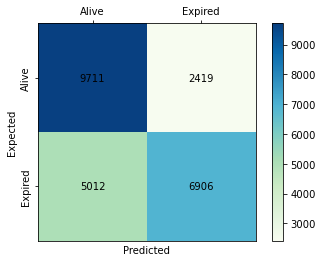
\includegraphics[width=8cm]{fig/chapter5/SVM/Confusion Matrix_new.png}
\caption{Confusion matrix for the \acrshort{SVM} algorithm}
\label{fig:svmconfusionmat}
\end{figure}

\begin{figure}[H]
\begin{tabular}{@{}cc@{}}
\begin{subfigure}{0.5\textwidth}
  \centering
  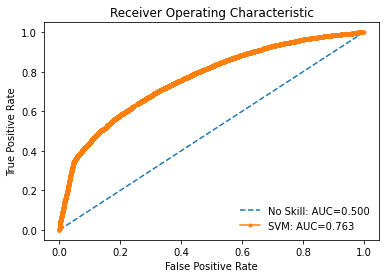
\includegraphics[width=7.5cm]{fig/chapter5/SVM/ROC_new.png}
  \caption{\footnotesize{The \acrshort{ROC} curve}}
  \label{fig:svmroc}
\end{subfigure} 
\begin{subfigure}{0.5\textwidth}
  \centering
  \includegraphics[width=7.5cm]{fig/chapter5/SVM/Precision-Recall_new.png}
  \caption{\footnotesize{The Precision-Recall curve}}
  \label{fig:svmprerec}
\end{subfigure} \\
\end{tabular}
\caption{Curves of \acrshort{ROC} and Precision-Recall using the \acrshort{SVM} algorithm}
\label{fig:svmcurves}
\end{figure}

\section{Implemented Logistic Regression Results}

\begin{table}[h]
\fontfamily{pcr}\selectfont
\centering
\setlength\tabcolsep{10pt}
\caption{\label{tab:lrreport}The classification report of the \acrlong{LR} algorithm}
\resizebox{0.7\textwidth}{!}{%
\begin{tabular}{@{}rrrrr@{}}
\thead{} & \thead{precision} & \thead{recall} & \thead{f1-score} & \thead{support} \\ [12pt]
Alive         & 0.66  & 0.75  & 0.70  & 12031       \\ 
Expired       & 0.71  & 0.61  & 0.65  & 12017       \\ 
                                                    \\
accuracy      &       &       & 0.68  & 24048       \\ 
micro avg     & 0.68  & 0.68  & 0.68  & 24048       \\
weighted avg  & 0.68  & 0.68  & 0.68  & 24048       \\
\end{tabular}}
\end{table}

\begin{figure}[H]
\centering
\includegraphics[width=8cm]{fig/chapter5/LR/Confusion Matrix_new.png}
\caption{Confusion matrix for the \acrshort{LR} algorithm}
\label{fig:lrconfusionmat}
\end{figure}

\begin{figure}[H]
\begin{tabular}{@{}cc@{}}
\begin{subfigure}{0.5\textwidth}
  \centering
  \includegraphics[width=7.5cm]{fig/chapter5/LR/ROC_new.png}
  \caption{\footnotesize{The \acrshort{ROC} curve}}
  \label{fig:lrroc}
\end{subfigure} 
\begin{subfigure}{0.5\textwidth}
  \centering
  \includegraphics[width=7.5cm]{fig/chapter5/LR/Precision-Recall_new.png}
  \caption{\footnotesize{The Precision-Recall curve}}
  \label{fig:lrprerec}
\end{subfigure} \\
\end{tabular}
\caption{Curves of \acrshort{ROC} and Precision-Recall using the \acrlong{LR} algorithm}
\label{fig:lrcurves}
\end{figure}

\section{Implemented Na\"ive Bayes Results}

\begin{table}[h]
\fontfamily{pcr}\selectfont
\centering
\setlength\tabcolsep{10pt}
\caption{\label{tab:nbreport}The classification report of the \acrlong{NB} algorithm}
\resizebox{0.7\textwidth}{!}{%
\begin{tabular}{@{}rrrrr@{}}
\thead{} & \thead{precision} & \thead{recall} & \thead{f1-score} & \thead{support} \\ [12pt]
Alive         & 0.60  & 0.92  & 0.73  & 12028       \\ 
Expired       & 0.83  & 0.39  & 0.53  & 12020       \\ 
                                                    \\
accuracy      &       &       & 0.65  & 24048       \\ 
micro avg     & 0.72  & 0.65  & 0.63  & 24048       \\
weighted avg  & 0.72  & 0.65  & 0.63  & 24048       \\
\end{tabular}}
\end{table}

\begin{figure}[H]
\centering
\includegraphics[width=8cm]{fig/chapter5/NB/Confusion Matrix_new.png}
\caption{Confusion matrix for the \acrlong{NB} algorithm}
\label{fig:nbconfusionmat}
\end{figure}

\begin{figure}[H]
\begin{tabular}{@{}cc@{}}
\begin{subfigure}{0.5\textwidth}
  \centering
  \includegraphics[width=7.5cm]{fig/chapter5/NB/ROC_new.png}
  \caption{\footnotesize{The \acrshort{ROC} curve}}
  \label{fig:nbroc}
\end{subfigure} 
\begin{subfigure}{0.5\textwidth}
  \centering
  \includegraphics[width=7.5cm]{fig/chapter5/NB/Precision-Recall_new.png}
  \caption{\footnotesize{The Precision-Recall curve}}
  \label{fig:nbprerec}
\end{subfigure} \\
\end{tabular}
\caption{Curves of \acrshort{ROC} and Precision-Recall using the \acrlong{NB} algorithm}
\label{fig:nbcurves}
\end{figure}

\section{Implemented LDA Results}

\begin{table}[h]
\fontfamily{pcr}\selectfont
\centering
\setlength\tabcolsep{10pt}
\caption{\label{tab:ldareport}The classification report of the \acrshort{LDA} algorithm}
\resizebox{0.7\textwidth}{!}{%
\begin{tabular}{@{}rrrrr@{}}
\thead{} & \thead{precision} & \thead{recall} & \thead{f1-score} & \thead{support} \\ [12pt]
Alive         & 0.65  & 0.76  & 0.70  & 12093       \\ 
Expired       & 0.71  & 0.59  & 0.65  & 11955       \\ 
                                                    \\
accuracy      &       &       & 0.68  & 24048       \\ 
micro avg     & 0.68  & 0.68  & 0.67  & 24048       \\
weighted avg  & 0.68  & 0.68  & 0.67  & 24048       \\
\end{tabular}}
\end{table}

\begin{figure}[H]
\centering
\includegraphics[width=8cm]{fig/chapter5/LDA/Confusion Matrix_new.png}
\caption{Confusion matrix for the \acrshort{LDA} algorithm}
\label{fig:ldaconfusionmat}
\end{figure}

\begin{figure}[H]
\begin{tabular}{@{}cc@{}}
\begin{subfigure}{0.5\textwidth}
  \centering
  \includegraphics[width=7.5cm]{fig/chapter5/LDA/ROC_new.png}
  \caption{\footnotesize{The \acrshort{ROC} curve}}
  \label{fig:ldaroc}
\end{subfigure} 
\begin{subfigure}{0.5\textwidth}
  \centering
  \includegraphics[width=7.5cm]{fig/chapter5/LDA/Precision-Recall_new.png}
  \caption{\footnotesize{The Precision-Recall curve}}
  \label{fig:ldaprerec}
\end{subfigure} \\
\end{tabular}
\caption{Curves of \acrshort{ROC} and Precision-Recall using the \acrshort{LDA} algorithm}
\label{fig:ldacurves}
\end{figure}

\section{Implemented KNN Results}

\begin{table}[h]
\fontfamily{pcr}\selectfont
\centering
\setlength\tabcolsep{10pt}
\caption{\label{tab:knnreport}The classification report of the \acrlong{KNN} algorithm}
\resizebox{0.7\textwidth}{!}{%
\begin{tabular}{@{}rrrrr@{}}
\thead{} & \thead{precision} & \thead{recall} & \thead{f1-score} & \thead{support} \\ [12pt]
Alive         & 0.92  & 0.69  & 0.79  & 12147       \\ 
Expired       & 0.75  & 0.94  & 0.83  & 11901       \\ 
                                                    \\
accuracy      &       &       & 0.82  & 24048       \\ 
micro avg     & 0.84  & 0.82  & 0.81  & 24048       \\
weighted avg  & 0.84  & 0.82  & 0.81  & 24048       \\
\end{tabular}}
\end{table}

\begin{figure}[H]
\centering
\includegraphics[width=8cm]{fig/chapter5/KNN/Confusion Matrix_new.png}
\caption{Confusion matrix for the \acrshort{KNN} algorithm}
\label{fig:knnconfusionmat}
\end{figure}

\begin{figure}[H]
\begin{tabular}{@{}cc@{}}
\begin{subfigure}{0.5\textwidth}
  \centering
  \includegraphics[width=7.5cm]{fig/chapter5/KNN/ROC_new.png}
  \caption{\footnotesize{The \acrshort{ROC} curve}}
  \label{fig:knnroc}
\end{subfigure} 
\begin{subfigure}{0.5\textwidth}
  \centering
  \includegraphics[width=7.5cm]{fig/chapter5/KNN/Precision-Recall_new.png}
  \caption{\footnotesize{The Precision-Recall curve}}
  \label{fig:knnprerec}
\end{subfigure} \\
\end{tabular}
\caption{Curves of \acrshort{ROC} and Precision-Recall using the \acrshort{KNN} algorithm}
\label{fig:knncurves}
\end{figure}

\section{Discussion}

\subsection{Comparison}
Given all the results for the seven different \acrshort{ML} algorithms, \crefrange{tab:cartreport}{tab:knnreport} and \crefrange{fig:cartconfusionmat}{fig:knncurves}, it is easy to deduce that \acrshort{XGB} outperforms the other algorithms. Even though our primary metric for model evaluation was \acrlong{AUC}, \acrshort{XGB} retains its supremacy in accuracy and \acrshort{AUC} in \textsc{Precision-Recall} curves. This outcome is achieved mainly because of the inherent power of the Decision-Tree-based algorithms in solving binary class problems, and also due to not having any missing data in our dataset along with applying \acrshort{SMOTE} to balance the skewed cohort. Figure \ref{fig:comparison} shows how much applying a resampling algorithm matters. When no \acrshort{SMOTE} is applied, \crefrange{fig:rskfoldnosmote}{fig:skfoldnosmote}, \acrshort{SVM} results in slightly better than the rest of the algorithms concerning \acrshort{AUC}. In contrast, when \acrshort{SMOTE} is employed, \crefrange{fig:rskfoldsmote}{fig:skfoldsmote}, \acrshort{XGB}, \acrshort{KNN}, and \acrshort{CART} become the premier models. It can also be derived from figure \ref{fig:comparison} that methods like \acrshort{LR}, \acrshort{LDA}, \acrshort{NB}, and \acrshort{SVM} are indifferent to \acrshort{SMOTE}, while \acrshort{KNN}, \acrshort{CART}, and \acrshort{XGB} are significantly affected by it.

\begin{figure}[H]
\begin{tabular}{@{}cc@{}}
\begin{subfigure}{0.5\textwidth}
  \centering
  \includegraphics[width=7.5cm]{fig/chapter5/Algorithm Comparison (no SMOTE, RSKFold).png}
  \caption{\footnotesize{Repeated 5-fold cross-validation without \acrshort{SMOTE}}}
  \label{fig:rskfoldnosmote}
\end{subfigure} 
\begin{subfigure}{0.5\textwidth}
  \centering
  \includegraphics[width=7.5cm]{fig/chapter5/Algorithm Comparison (no SMOTE, SKFold).png}
  \caption{\footnotesize{Ten-fold cross-validation without \acrshort{SMOTE}}}
  \label{fig:skfoldnosmote}
\end{subfigure} \\
\begin{subfigure}{0.5\textwidth}
  \centering
  \includegraphics[width=7.5cm]{fig/chapter5/Algorithm Comparison (SMOTE, RSKFold).png}
  \caption{\footnotesize{Repeated 5-fold cross-validation with \acrshort{SMOTE}}}
  \label{fig:rskfoldsmote}
\end{subfigure} 
\begin{subfigure}{0.5\textwidth}
  \centering
  \includegraphics[width=7.5cm]{fig/chapter5/Algorithm Comparison (SMOTE, SKFold).png}
  \caption{\footnotesize{Ten-fold cross-validation with \acrshort{SMOTE}}}
  \label{fig:skfoldsmote}
\end{subfigure} \\
\end{tabular}
\caption{Comparison of the algorithms based on the \acrshort{AUC} criterion with/without \acrshort{SMOTE}}
\label{fig:comparison}
\end{figure}

{\hskip 1em} Figure \ref{fig:comparison} can also be analyzed from another point of view. Due to its synthetic behavior, utilizing \acrshort{SMOTE} balances the dataset in such a way that the \textit{Standard Deviation} of each algorithm is by far less than when no \acrshort{SMOTE} is used.

{\hskip 1em} Aside from confusion matrix, accuracy, and the \acrshort{AUC}, there is another classification evaluation method called \textbf{Cohen's Kappa}, a statistic to test interrater reliability, i.e., the extent of agreement among data collectors \cite{mchugh_interrater_2012}. Table \ref{tab:cohenskappa} demonstrates the value of Cohen's Kappa for each method. It can be seen that considering this criterion, \acrshort{XGB} achieves the highest Cohen's Kappa, which makes it the best algorithm among the rest.

\begin{table}[H]
\centering
\setlength\tabcolsep{50pt}
\caption{\label{tab:cohenskappa}Calculated Cohen's Kappa for the implemented models}
\begin{tabular}{@{}lc@{}}
\toprule
\thead{Algorithm}     & \thead{Cohen's Kappa}        \\ \midrule \midrule
\acrfull{CART}        & 0.683919                     \\ \midrule
\acrfull{XGB}         & 0.803587                     \\ \midrule
\acrfull{SVM}         & 0.380761                     \\ \midrule
\acrfull{LR}          & 0.359726                     \\ \midrule
\acrfull{NB}          & 0.308094                     \\ \midrule
\acrfull{LDA}         & 0.352173                     \\ \midrule
\acrfull{KNN}         & 0.672806                     \\
\bottomrule
\end{tabular}
\end{table}

\subsection{Computational Complexity}
There is another aspect of studying \acrlong{ML} algorithms and evaluating them: Computational Complexity, which gives an asymptotic upper bound to a function and is referred to as big-O notation. It bounds the growth of the running time from above and describes the code complexity using algebraic terms \cite{kearns_introduction_1994}. Table \ref{tab:bigonotation} shows the formulated computational complexity for the algorithms used in our work. \

{\hskip 1em} In calculating the big-O notation, only dominant terms, and not coefficients, matters. Regarding that, the common term in all the formulas of table \ref{tab:bigonotation} is $n$, which is the input size ($n=59190$). $d$ denotes the number of dimensions or features ($d=11$). In \acrshort{KNN}, parameter $k$ is the number of nearest neighbors taken into account ($k=25$), while in \acrshort{XGB}, it means the number of trees ($k=100$). Eventually, ${\lVert\mathrm{x}\rVert}_0$ stands for the number of non-missing entries in the training data (${\lVert\mathrm{x}\rVert}_0=59190$).

{\hskip 1em} Table \ref{tab:complexitytime} represents the running time of a single instance of the training set of each implemented algorithm. It can be recognized that \acrshort{SVM} has the longest running time that is understandable since it uses an internal five-fold cross-validation, which increases the running time exponentially. From the big-O notation point of view, it can also be concluded since the \acrshort{SVM} behavior corresponds to $n^2$, and $n$ is quite huge. Comparing an algorithm's big-O notation formula with its respective instance running time, considering the parameter values, proves that the calculated running times are as rational as expected.

\begin{table}[H]
\centering
\setlength\tabcolsep{50pt}
\caption{\label{tab:bigonotation}Training computational complexity of the algorithms}
\begin{tabular}{@{}lc@{}}
\toprule
\thead{Algorithm}     & \thead{Big-O Notation}        \\ \midrule \midrule
\acrfull{CART}        & $O(nlog(n)\times d)$          \\ \midrule
\acrfull{XGB}         & $O(kd{\lVert\mathrm{x}\rVert}_0log(n))$   \\ \midrule
\acrfull{SVM}         & $O(n^2)$                      \\ \midrule
\acrfull{LR}          & $O(nd)$                       \\ \midrule
\acrfull{NB}          & $O(nd)$                       \\ \midrule
\acrfull{LDA}         & $O(nd^2)$                     \\ \midrule
\acrfull{KNN}         & $O(nd+kn)$                    \\
\bottomrule
\end{tabular}
\end{table}

\begin{table}[H]
\centering
\setlength\tabcolsep{30pt}
\caption{\label{tab:complexitytime}The running time of a single training set instance}
\begin{tabular}{@{}lc@{}}
\toprule
\thead{Algorithm}     & \thead{Instance (ms)}         \\ \midrule \midrule
\acrfull{CART}        & 0.00405                       \\ \midrule
\acrfull{XGB}         & 0.42355                       \\ \midrule
\acrfull{SVM}         & 16.7944                       \\ \midrule
\acrfull{LR}          & 0.02082                       \\ \midrule
\acrfull{NB}          & 0.00162                       \\ \midrule
\acrfull{LDA}         & 0.00282                       \\ \midrule
\acrfull{KNN}         & 0.00615                       \\
\bottomrule
\end{tabular}
\end{table}
\providecommand\phantomsection

\chapter{Conclusion}\label{chap:conclusion}

\acrfull{ML} in medicine has been around for years, with the aim of medical treatment. This thesis focuses on the decision support aspect of \acrshort{ML} to present a model that can precisely predict mortality by means of the utilization of some relevant features. \

{\hskip 1em} \acrfull{eICU-CRD} is chosen as our study resource. A database, which comprises 31 tables and over 457 million rows of measurements. Despite performing a thorough analysis of its demo version, only four tables, \textit{apachePredVar}, \textit{infusionDrug}, \textit{patient}, and \textit{lab}, were selected to build our cohort due to some hardware limitations. Ultimately, a 59190-row dataset including age, gender, weight, glucose values, lactate values, diabetes, and mortality was created for further implementation. \

{\hskip 1em} Seven \acrlong{ML} algorithms have been applied to our dataset, and the results of each have been extracted. Finally, it is shown that regarding criteria such as accuracy, \acrshort{AUC} for both ROC and \textsc{Precision-Recall}, and Cohen's Kappa, \acrfull{XGB} outperforms the other. All the algorithms were also discussed in terms of Training Computational Complexity, and it can be seen that \acrshort{SVM} has the longest running time by far. \
\providecommand\phantomsection

\chapter{Future Work}\label{chap:future}

In this thesis, mortality prediction was studied based on patients' glucose and lactate values. However, there is a huge potential in medicine to analyze clinically ill patients from different perspectives, such as:

\begin{itemize}
    \item \textbf{Multi-class:} One aspect of analyzing clinical databases like \acrshort{eICU-CRD} is to consider more than a single binary outcome (in our work, mortality). Adding more output features increases the dimension and, therefore, the complexity of the cohort analysis, and perhaps, the need for utilizing Deep Learning rises. 
    \item \textbf{Time:} One of the most interesting features to be added to our study is time. Considering the time allows us to better track a patient's situation, improved estimate when they need medication or operation, better follow and study the vital signals trend, and better predict the death's probable time. Take into account that most clinical databases use irregular time series as in \acrshort{eICU-CRD}.
    \item \textbf{Real-time implementation:} Once the implementation has been tested and approved, it can be used in real-time databases to make the predictions practical, like what is currently happening in \textit{Telemedicine}.
    \item \textbf{\acrlong{NLP}:} There are tables in \acrshort{eICU-CRD} like the \textit{nurseCharting} table which consists of nurse-entered information that can give much information about the patient's disease. Nevertheless, in order to extract them, \acrshort{NLP} is needed.
    \end{itemize}
\providecommand\phantomsection

\cleardoublepage\phantomsection\addcontentsline{toc}{chapter}{References}
\printbibliography[title={References}]

%\cleardoublepage\phantomsection\addcontentsline{toc}{chapter}{Glossary}
\printglossary[title=Glossary, type=\acronymtype]

\end{document}